\Chapter{Life on Athas}
{Almost all the Tyr Region is a desert wasteland, though it is beautiful and spectacular in its own fashion. Over each hill, behind each sand dune, the terrain appears more awesome than the land before. In my travels, I have often been overwhelmed by the sheer magnitude of this land, cowed by its indifferent brutality, even frightened by the unrestrained might of its elements---but I have never been bored.

Can I impart the grandeur and majesty of this area with mere words? I wonder. I can describe the queasy feeling of sliding down the glassy slopes of the Smoking Crown, or make your eyes sting with tales of walking the salt flats on a windy day. My words are but transparent reflections of this magnificent land, but perhaps they can be of use.}
{The Wanderer's Journal}

\Capitalize{A}{thas} is still a largely unknown world. Millennia of misinformation, wars, and natural barriers have created isolated pockets of civilization between large expanses of desert terrain.

The known world is currently divided into the Silt Sea, the Tablelands (also known as the Tyr Region), the Ringing Mountains, and the Hinterlands. The Tyr Region is defined as the area bordered by the Sea of Silt on the east, the Hinterlands to the west, and the Endless Sand Dunes to the south.

Outside of those regions, the Jagged Cliffs, the Deadlands, and the Valley of the Cerulean Storm wait to be discovered, charted, and plundered. The surface of Athas stretches from horizon to horizon, a patchwork of fields and forests, oceans (of water and sand) and mountains, deserts, swamps, jungles, and more. Beneath the crimson sun, Athas' varied environments give way one to another across the Tablelands. Mountains rise, valleys fall, and desert surrounds the land.

\section{The World of Athas}
Athas is a desert-sun-scorched and wind-scoured, parched and endless, but that does not mean that the landscape is monotonous. Far from it; over each hill, behind each dune, the terrain is more awesome, more spectacular, and more beautiful than any one has seen before. North or south, east or west, Athas contains natural wonders and dangers undreamed of on other worlds.

Storms blow in from the Sea of Silt, walls of pearly dust billow three thousand meters into the air, then come roiling ashore like a mountain range crashing down about unwary travelers. There are hundreds of different kinds of terrain on Athas, from wind-scoured pebble flats to twisted badlands canyons to gleaming sands to jumbled boulder fields.

In this chapter, the world of Athas is examined from the point of view of the Tablelands, also known as the Tyr Region, the region that has influenced Athas (for good or bad) the most.

\subsection{Time}
Each year is made up of exactly 375 days: the exact time between highest suns. Athasians have no seasons that govern their thinking of time, for there is no marked difference in temperature or weather patterns. However, the year is divided into three equal phases: High Sun, Sun Descending, and Sun Ascending. Highest sun is the first day of the year, and lowest sun indicates the midpoint of the year (which, incidentally, occurs at midnight and is generally observed in night-time ceremonies).

\subsection{Marking the Years}
Every city-state and merchant house has its own calendar, but the most commonly used is the Calendar of Kings. In the Calendar of Kings, years are counted off using a pair of concurrently running cycles: one of eleven parts, the other of seven. The eleven-part, or Endlean cycle, is counted and spoken first, in the order presented below. The seven-part, or Seofean cycle, is counted and spoken second. The Endlean cycle is complete when Athas' two moons, Ral and Guthay, meet in the heavens, resulting in a major eclipse that occurs every 11 years. The Seofean cycle is more abstract, occurring after Agitation has led back to Fury in the cosmos.

Every 77 years the cycle repeats itself, ending with a year of Guthay's Agitation and starting again with a new year of Ral's Fury. Each 77-year cycle is called a King's Age. There have been 189 complete King's Ages since this calendar was adopted more than 14,500 years ago.

So, the first year of each King's Age is a year of Ral's Fury. The next year is a year of Friend's Contemplation, etc. The 76th year of each King's Age is a year of Enemy's Reverence, followed by the 77th year, a year of Guthay's Agitation.

\Table{Calendar of Kings}{C C}{
\tableheader Endlean Cycle & \tableheader Seofean Cycle\\
Ral & Fury\\
Friend & Contemplation\\
Desert & Vengeance\\
Priest & Slumber\\
Wind & Defiance\\
Dragon & Reverence\\
Mountain & Agitation\\
King &\\
Silt &\\
Enemy &\\
Guthay &\\
}

While each city-state has its own official calendar, the dynastic merchant houses have, over the centuries, come to use a standardized book of days. This has evolved slowly over time as the need to efficiently coordinate activities with trading partners grew. The calendar is generally referred to as the Merchant's Calendar. In the cities, it usually bears the name of the largest merchant house (which also generally receives the credit for inventing it).

The Merchant's Calendar divides the 375-day year into three 125-day seasons---High Sun, Sun Descending and Sun Ascending. Each season is divided into four 30-day months made up of six day weeks. A five day long festival week in the middle of each season lies outside the confines of the months.

The year begins on the day of Highest Sun, midway through the season of High Sun.

\Table{Merchant's Calendar}{l l c X}{
\tableheader Season & \tableheader Month & \tableheader Days & \tableheader Star Sign\\
High Sun & Dominary & 30 & Balimarash the Caravan\\
High Sun & Sedulous & 30 & Fiddle the Beetle\\
Sun Descending & Fortuary & 30 & Hesper the Kenku\\
Sun Descending & Macro & 30 & Saurus the Lizard\\
Sun Descending & Dessalia & 5 & On the cusp\\
Sun Descending & Fifthover & 30 & Hortle the Spider\\
Sun Descending & Hexameron & 30 & Sylk the Wyrm\\
Sun Ascending & Morrow & 30 & Tasker the Scorpion\\
Sun Ascending & Octavus & 30 & Pyrus the Wheel\\
Sun Ascending & Assalia & 5 & On the cusp\\
Sun Ascending & Thaumast & 30 & The Dragon\\
Sun Ascending & Anabasis & 30 & Tyrospur the Lion\\
High Sun & Hoard & 30 & Scratch the Basilisk\\
High Sun & Flagstaad & 30 & Krawler the Kank\\
High Sun & Zenalia & 5 & On the cusp
}
\City{Balic}
{28,000 (78\% humans, 8\% dwarves, 4\% elves, 4\% half-giants, 3\% muls, 2\% thri-kreen, 1\% other).}
{Grain, salt, olives, kank nectar, leather, livestock, silver.}
{Common, Dwarven, Elven, Balikite.}
{
\Figure{b}{images/balic-1.png}

	The sorcerer-king Andropinis once ruled Balic from the airy confines of the White Palace, not far from the dusty shores of the city's silt harbor. One day in the Year of Friend's Agitation (FY 10), he boarded his silt armada and struck out for the far side of the Sea of Silt. It was a trip from which he never returned.

	Balic has suffered on a number of fronts in recent years. In the Year of Dragon's Agitation (FY 3), when Tyr had refused to pay the Dragon's Levy, it fell to Balic to make up the loss by adding an extra thousand slaves to its contribution. The following year, Mountain's Fury, saw the Peninsula Rampage, a short-lived war in which a small army of giants overran most of the Balican Peninsula. Half of Balic's army and a quarter of its fields were destroyed in the battle. The city-state was still recovering when Andropinis fell to Rajaat's revenge a few years later.
}
{
	Balic is a clean, comfortable metropolis on the shores of a silt bay. Since Andropinis' disappearance, the city has been divided into three parts, each ruled over by a different trade lord. Balic was untouched by the Great Earthquake, but other disasters have left their marks on the place in recent years. For the most part, however, life under the trade lords is considerably better than it was under the cruel and oppressive Andropinis.

	Even the territory controlled by House Tomblador, whose lord attempts to pattern himself as Balic's new dictator, is pleasant compared to the atrocities of the previous ruler.

	On the surface, the city appears to be one sprawling metropolis, not a divided city. No walls separate one territory from another, no guards wait to collect tolls as citizens move from block to block. To the locals, however, there is a clear delineation between one lord's domain and the next. Wavir is free and bright, Tomblador oppressive and dark, and Rees is like an extended work camp where everyone labors for the benefit of the trade lord.

	Though they appear to cooperate for the good of the city, the trade lords wage a secret war against each other that everyone knows about but few people understand. None of the trade lords is willing to let this conflict escalate into a full-scale civil war, but they have come very close to it in recent months. Caravans have been raided or sabotaged, warehouses plundered or burnt to the ground, and important agents have been killed on all sides. How far each is willing to push before a better solution must be found remains to be seen.

	To stave off another war with the giants, House Rees has sent representatives into the silt basin to negotiate a lasting peace. No contracts have been agreed upon, but it seems Balic may soon have an agreement with the usually hostile giants.

	The three contenders for rulership of Balic before the trade lords made their moves are still active in the city-state. Oriol the Patrician has dedicated his noble house to Lord Tabaros; though he is ready to step back to the forefront should the old man grow too sick to rule. General Zanthiros has fled the city with a small but significant portion of the city militia. His band operates as a raiding tribe along the peninsula, waiting for an opportunity to return to Balic to seize power. The templar Asthira, meanwhile, has gone into hiding within the city. From her place in the shadows, she continues to keep in contact with many of the templars who still have roles in the government, as well as with those who have taken to hiding. She hopes to eventually overthrow the trade lords, who she feels illegally took power.

	Dark rumors persist that Andropinis is able to contact his loyal templars (such as Asthira) from his prison in the Black. These can be neither confirmed nor denied at this time, but the thought of Andropinis continuing to exert influence over the city has the local Veiled Alliance more than a little concerned. If the rumors are true, is Andropinis working with his exiled templars or with someone currently in power somewhere in the city?
}
{
\Figure*{b}{images/balic-2.png}

	After Andropinis' imprisonment, Balic was divided into three parts, each controlled by a different trade lord. These parts cooperate on one level but battle for supremacy on all others.

	The largest block of control falls to Lord Tabaros of House Wavir (NG male human, aristocrat 7/rogue 8/dune trader 5), while Lord Kaladon of House Tomblador (LE male human, rogue 8/dune trader 5) and Lady Essen of House Rees (LN female human, rogue 7/dune trader 5/telepath 4) control equally sized smaller blocks. The same amount of cooperation that allows the three rivals to jointly maintain the major trading village of Altaruk allows them to keep Balic running as a major city-state.

	As far as outsiders are concerned, the three leaders formed a triune council to rule the city after Andropinis fell. While such a council does exist, and the three rivals meet regularly to keep the city-state strong enough to stand against invaders, they each work behind the scenes to build their own power bases up and knock their rivals down.

	Each trade lord has a different view of the world and the way Balic should be governed. Wavir, for example, wants to free all slaves, outlaw defilers, welcome preservers into society, and set up a true democratic state. The way to accomplish this, Lord Tabaros believes, is by quick action and harsh measures. Unfortunately, Tabaros is more than 100 years old and may not be able to stay in power much longer. Publicly, the trade lord appears as sharp and healthy as ever, but privately he suffers the weaknesses of age and illness. He had hoped to pass leadership to his son long ago, but his son died when raiders attacked his caravan in FY 6. The next likely candidate, Tabaros' granddaughter Tarinne (NG female human, fighter 4/rogue 2/dune trader 4), isn't ready for the responsibilities yet (or so Tabaros believes).

	Lord Kaladon wants to resume the dictatorship---with himself as king of Balic. Lady Essen, meanwhile, believes that the city-state should be nothing more than a glorified merchant village, serving to fill the coffers of House Rees and making it the most powerful merchant house in the entire Tyr Region. Needless to say, none of the sides want to see any other gain a significant advantage.

	Those templars who agreed to swear allegiance to one of the trade lords have been retained for their bureaucratic skills. However, the merchant houses have their own administrators to fall back on, so any templars who can't be trusted are eliminated. (A small number of templars still loyal to Andropinis have gone into hiding and continue to work in secret, though they have little power and few hopes of gaining any under the current system.)

	The patricians are allowed varying degrees of participation in the government, depending upon which merchant house holds sway over the territory their land occupies. Under Wavir's control, the patricians are allowed full participation rights. Under House Tomblador, the patricians are treated barely better than slaves, while House Rees gives them the freedom to handle their own affairs-provided they meet the production quotas Lady Essen has established for each patrician family.
}
{
	Today the city-state has no sorcerer-king to lead it or protect it from the ravages of Athas. Balic has always had a tradition of the illusion of democracy. Andropinis claimed to have been freely elected to his position, the templars were elected to ten-year terms by the free citizens, and even the nobles (called patricians) were allowed to participate in the governmental process by selecting members to attend the Chamber of Patricians on a regular basis. Though this democracy wasn't real, it still taught the people about one possible way a free society could work. When the news spread that Andropinis was gone (he had been imprisoned in the Black by Rajaat), various factions called for a new election.

	The main contenders for the position of dictator of Balic were Oriol of Magestalos, First Speaker of the Patricians (LN male human, telepath 7); General Zanthiros of the Balican army (LE male human, fighter 13); and First Templar Asthira (LE female human, templar 6/shadow templar 7). Before the final votes could be counted, Tabaros, the patriarch of House Wavir, made his move. The merchant house seized the White Palace, the silt harbor, and all of the territory in between and declared Tabaros to be the Trade Lord of Balic. This didn't sit well with House Wavir's rivals. Neither House Tomblador nor House Rees wanted to be cut out of this opportunity, so each of these merchant dynasties took over the remaining portions of the city.

	\textbf{Shadow Templars:} When the Trade Lords seized power in Balic, many of the templars swore allegiance to one of the Trade Lords. A small number of templars refused to abandon their loyalty to Dictator Andropinis and have gone into hiding. They hope to one day free Andropinis from his prison, and there are rumors that the shadow templars have already developed a means of communicating with the imprisoned sorcerer-king. They work in the shadows, but have many contacts with the templars that have pledged their allegiance to the Trade Lords. First Templar Asthira leads the shadow templars.

	\textbf{The Veiled Alliance:} Like other organizations in Balic, the city's Veiled Alliance is run by an elected leadership. For this reason, a nonwizard leads the Alliance. Ramphion (LG male human, rogue 11) has held his position for 15 years, winning five elections in a row. The next election must occur later this year, and Ramphion may finally give up his role as head of the Alliance. He has strong ties to House Wavir, though House Rees has begun to court the preservers. Ramphion listens to all sides, hoping to play peacemaker if the three factions ever resort to civil war. The Alliance has two other goals at the moment: to turn Balic into a true democratic society, and to find out if the rumors concerning Andropinis are true.
}
{
	\textbf{Altaruk (Village, 620):} Altaruk is a client village of the merchant houses of Wavir, Rees, and Tomblador. This major trade village is located at the head of Big Fork of the Forked Tongue Estuary. Heavily fortified, a 4.5-meter wall surrounds the village, and 500 free mercenaries defend it. Altaruk is commanded by Arisphistaneles (LG male human, wizard 5/veiled one 6/dune trader 4), a powerful preserver who allows the Veiled Alliance to use the village as a meeting place. The village is regularly attacked by giants from the islands of the Forked Tongue, and the Great Earthquake buried parts of Altaruk beneath rubble from the nearby mountains. As always, the merchant houses of Balic are in the process of rebuilding the village, for it serves as a key deterrent to raiders along this portion of the trade roads. Protection is extended to caravans of other merchant houses, provided they pay the toll as they pass through Altaruk. For caravans, the toll is one gold piece per caravan mount, an exorbitant price that prohibits most merchants from spending more than one day in the village. For individual travelers the toll is one ceramic piece.

	\textbf{Last Port (Hamlet, 200):} The village of Last Port is surrounded by a silt moat. The village falls under the influence of Balic, but has maintained its independence as much as it can. Aicmenes (LN male human, telepath 9) leads the village. The village is a mix of Dwarven architecture, influenced by the Smokestone clan that makes Last Port its home, and Balic artistry. A small amber mine is the main source of income for the village, though many villagers also provide services for the silt skimmers that stop at the village's small docks.

	\textbf{Walis (Thorp, 120):} Walis is a small hidden village in the foothills of the Ringing Mountains. From its position atop a high rock spire the village sits on one of the only active gold mines in the Tyr region. The merchant house Tomblador controls the village and keeps the village's defenses as strong as possible. The village can only be reached from the ground by a cargo bucket lowered by the villagers. Besides a large company of soldiers, six defilers are stationed at the village at all times to add to the defenses.
}
{
	\textbf{Agora:} All the merchant houses have their emporiums in the Balican agora. Surrounding the agora is the Elven market.

	\textbf{Criterion:} Balic's gladiator arena sits beneath the stony bluff of the Megaleneon. The Criterion is an architectural marvel, constructed of pure white marble, with great sails rising from the walls to provide shade. The arena floor is rectangular shaped and consists of hexagon-shaped marble slabs. The slabs are 3 meters wide and 9 meters tall and rest on a bed of sand. This unique floor is always uneven since no two adjoining slabs are of the same height, with as much as 3 meters difference between two slabs.

	\textbf{Fort Glamis:} Established and maintained by House Wavir, Fort Glamis is located on the Balic/Ledopolus road and is an important supply center for caravans from Balic on their way to the rest of the Tyr region.

	\textbf{The Shining Bridges:} Ravines, filled with silt, break through the ground around the agora. Monumental bridges made of marble allow access to the agora.

	\textbf{Segovara:} The village of Segovara was a client village of House Rees of Balic. Located southeast of Balic across the Estuary of the Forked Tongue, the village rests inside a small narrow canyon. The village is mainly a collection of huts built against both sides of the canyon walls. Because of the lack of space inside the canyon only one narrow road exists in the cramped village. The villagers manufactured leather goods for House Rees, however their isolated position, without a source of water, left them utterly depended on Rees caravans. In the chaotic aftermath of the trade lords' seizure of power in Balic the village was forgotten and all of the villagers perished. The next time a caravan from House Rees arrives at the village the entire population will rise as faels.
}
{
	\item Working in secret, a group of templars attempts to open a portal to Andropinis' prison in the Black. Unfortunately for the templars, they were duped by an extraplanar creature into opening a portal to its plane, allowing a band of extraplanar creatures onto Athas. These creatures proceed to run amok throughout Balic. The creatures could be from the Black, one of the elemental planes, or another plane of the DM's choosing.
	\item The animals on House Dagsonius's ranch have begun to talk! The animals do not respond to spoken questions, but randomly blurt out predictions of doom in perfect Balikite to those standing nearby. The head of House Dagsonius is troubled. He raises the animals for slaughter but many in the family do not want to kill the animals if they have become intelligent. He needs someone to get to the bottom of this.
	\item Drake Crag Bay is not far from Balic and takes its name from a rocky crag overlooking the bay that resembles an earth drake. For years the bay has been a prime spot to harvest silt mussels, and many from Balic make their livelihood in the shallow bay. Recently a creature from the deep silt has entered the bay and preys on the mussel harvesters. The creature has remained under the silt so far, so no one is sure what the creature is.
	\item With the current struggle for control of Balic between the three merchant houses being mostly a war in the shadows, the bards of Balic are taking advantage of all sides to generate high profits. When the PCs show up in town, a few of the bards see them as mercenaries who could become competition. The bards try to either force the PCs out of town or eliminate them.
	\item The Silt Blazer, a silt skimmer based out of Balic was three days overdue when it finally sailed into Balic harbor---with no one aboard. There is no sign of the crew; however, the skimmer's cargo appears to be intact. While House Wavir has confiscated the cargo, they hired the PCs to find out what happened to the crew.
	\item As a sign of his status as Dictator, Andropinis did not wear a crown. His position was signified by a rod and cloak, both rumored to be enchanted. The royal regalia disappeared from the Megaleneon in the days after the trade lords seized power. All three trade lords desire the royal regalia to strength their claim to rulership of the city and will pay handsomely for any who recover the items.
}
\City{Draj}
{15,000 (60\% humans, 15\% dwarves, 15\% elves, 5\% muls, 3\% half-elves, 2\% half-giants).}
{Wheat, rice, hemp, livestock, textiles, straw mats, pottery.}
{Common, Dwarven, Elven, Draji.}
{
	Draj, situated on a vast mud flat east of Raam, was another warlike city-state before its sorcerer-king was killed by Rajaat during his brief escape in FY 10. Before the news could cause panic and social upheaval in the city, King Tectuktitlay's templars (called ``moon priests'') quickly took stock of the situation, trying to find some way to preserve immortal Draj. The templars knew they had no real power without the spells granted by their sorcerer-king, so the supreme moon priests approached the most powerful masters of King Tectuktitlay's psionic academy, the House of the Mind. After numerous secret meetings, a plan was hit upon: The rulership of Draj would pass on to King Tec's ``son,'' a young psionicist named Atzetuk.

	The masters of the Way altered the teenager's mind, making him believe he was actually the king's son. Then they instructed him on what to say to the city's masses to instill confidence. In reality, the templars and psionic masters would share rulership of the city, working behind the scenes while the populace looked upon young Atzetuk as their new god-king. The transition from one king to another was accomplished quite easily; order had never been a problem in Draj, as its citizens were enraptured with the theocracy and religious trappings Tectuktitlay had surrounded himself with. As such, it was an easy task for the templars to use these rituals to save the city and keep the government running smoothly.
}
{
	Draj's citizens dress in loose, bright-colored shirts and skirts. All citizens wear headdresses of some sort, usually a roll of cloth or giant-hair braids, though the wealthy go in for more elaborate designs. By law only warriors may wear more than a single feather.

	The war festivals and religious ceremonies dedicated to the twin moons of Athas are the focus of life in Draj. The people have lost a god-king they neither respected nor believed in, but have gained a new god-king that is both well liked and inspires faith and reverence. This has surprised the secret leaders of the city, though not to the point where they have grown concerned. If their plan to replace King Tectuktitlay has succeeded beyond their wildest dreams, so much the better. Life in Draj remains the same as always---only the name of the king has changed.

	The natural disasters of the west never reached Draj. Rumors of a Great Earthquake arrived with the passing traders, but not even the slightest tremor or quake disturbed the city. Draj was inundated by one of the first Tyr-storms, however. The mud fields flooded, ruining crops and killing more than a few Draj citizens before the rain stopped falling and the wind and lightning abated.

	It didn't take long for the templars to clean up in the wake of the storm or for King Atzetuk to assuage the fears of his citizens. He called for sacrifices to appease the elementals, and the people of Draj approved. Atzetuk sent his warriors out into the wilderness to find captives worthy of dying on Draj's great pyramid, and before the week had passed rivers of blood washed over the pyramid's stone steps. Because of the relative closeness of the Cerulean Storm and because the Tyr-storms often pass within sight of Draj as they sweep inland, the sacrifices have become a regular ritual. The citizens believe that the blood will keep the storms at bay-after all, that's what their king has told them.

	The problems in Raam have had an effect on Draj. The templars and psionic masters watch the unfolding events as omens of what could occur in Draj if the illusion they've woven around Atzetuk ever unravels. Plus, many refugees have fled Raam and sought sanctuary in Draj. Most of these expatriates found only death, either in the mud flats or atop the bloody pyramid at the heart of the city. At some point, these lost exiles will find a voice and shout their grievances-and perhaps the citizens of Draj will hear that shout. The secret leaders fear Draj's society will collapse if the people lose faith in King Atzetuk.

	Atzetuk himself poses another problem for Draj's secret leadership. Every day, the youth gains more and more confidence. His belief in his own divinity strengthens.

	Soon, the masters of the Way suspect, they will lose control of the youth. While they don't want Draj to be overcome by anarchy and violence, they also don't want to give up the authority they've gained since Tectuktitlay's death. If Atzetuk continues to assert himself, the masters of the Way and the moon priests might decide to remove the king they put in place. After all, they reason, Draj survived the death of one king. It will surely survive the death of a second.
}
{
	Atzetuk (NG male human, telepath 6) apparently rules Draj, but he's nothing more than a figurehead who sits on the throne and carries on the practices and traditions of war set forth by King Tectuktitlay. The youth is paraded before his subjects every day and holds court in the Father and Master Temple. Although Atzetuk believes he's the legitimate heir to Tectuktitlay's throne and the true ruler of Draj, the business of government is managed by the moon priests and the masters of the House of the Mind. The templars have some power in this alliance, but the real leaders of the city are the masters of the Way, who bow to the commands of old lxtabai the Blind (LN male human, egoist 12). It's in everyone's interest to maintain this illusion. Without the young god-king, the nobles and free citizens would rebel against the rule of templars and mindbenders.

	Draj's noble families participate in the governing of the city through special meetings held at tecpans. In these long buildings, noble elders gather to debate and resolve problems considered too ordinary and routine to concern the moon priests and the new god-king. The noble elders are all great warriors. They will follow Atzetuk for as long as the warrior traditions and ceremonies are upheld.
}
{
	\textbf{Knights:} There are a number of knightly orders that are part of the Draji society. The two most important are the eagle knights and the jaguar knights. The eagle knights are among the most brutal and fanatical Draji warriors and rank second behind only the jaguar knights. The jaguar knights are the finest warriors of Draj. They undergo intense training to conquer their fear and strike fear in their opponents.

	\textbf{House Tsalaxa:} The merchants of House Tsalaxa conduct most of the trade for the city of Draj. Tsalaxa is known for its ruthless practices, well suited for a warrior culture. These traders regularly engage in espionage and intrigue in order to secure valuable contracts and business opportunities. The new head of the House, Yarsha Tsalaxa (LN female human, aristocrat 2/rogue 15), has some private doubts about the legitimacy of Atzetuk's rulership. However, she's still trying to settle her own position as leader of House Tsalaxa in the wake of her grandfather Ydris' death, and she doesn't want to express her concerns without solid proof to back them up. In the meantime, she'll continue to aggressively control the merchant house and keep the trade routes active and open to benefit the city and fill her own coffers.

	\textbf{The Veiled Alliance:} Draj's Veiled Alliance is hampered by poor leadership and indecisiveness. The current leader, Chimali Zaachila (LG female human, preserver 5), pretends to be much more powerful than she really is. Her lack of ability and training makes her reluctant to launch any daring programs that might reveal her secret. As such, the Alliance has no spies in high places, no active programs designed to thwart the king and his templars, and no plans to accomplish anything of lasting importance. The Alliance in Draj does offer some assistance to visiting preservers, but has little else to make it much more than a secret club for wizards.
}
{
	\textbf{Break Shore (Village, 100):} Break Shore is a trading village on the shore of the Silt Sea. Originally a client-village of Raam, the Draji gained control over the village during a war between the two city-states centuries ago, when gold was discovered in the nearby Mastyrial Mountains. The gold mine has been nearly depleted, though Draji templars still supervise bands of slaves struggling to uncover any little bit of precious metal remaining.

	\textbf{Bitter Well (Village, 100):} Bitter Well is located on the shore of the Silt Sea. Originally built by dwarves the village's buildings are made of stone, and a grand well lies at the center of the village. The buildings are packed close together and canvas drapes are hung between them to provide shade. However, the drapes also create a closed environment and traps the smell of unwashed bodies in the streets.

	\textbf{Ket (Village, 500):} The village of Ket is located on a small mud flat completely surrounded by an inland silt basin. The only way to access the village is along a mile-long causeway. The village maintains lucrative grain fields, which have maintained the village for years. With the renewed contact with the city-states of the North, Ket is becoming an important stop for caravans on the way north from Draj, bringing more prosperity the villagers.
}
{
	\textbf{Father and Master Temple:} More often known just as the Great Pyramid, the Father and Master Temple is a grand pyramid of stone and marble that is easily the largest building in Draj. The Great Pyramid houses administrative offices as well as the King's private quarters. Treasure rooms are rumored to fill the lower levels of the pyramid.

	\textbf{Fort Ebon:} Fort Ebon is a major supply point for all Tsalaxa's caravans traveling west from Draj. Located between Draj and Raam, all of the House's caravans that travel to the other city-states of the Tyr region stop at the fort.

	\textbf{Fort Firstwatch:} A merchant fort owned by House M'ke, Firstwatch is a supply point mid way between Raam and Draj. The fort defenders see frequent raids by elf nomads and mercenaries hired by rival houses, especially House Tsalaxa.

	\textbf{Fort Ral:} Fort Ral is a supply route on the road north from Ket. The fort was built on the ruins of an ancient pyramid. A contingent of soldiers from Draj, mostly archers, garrisons the fort. The soldiers patrol the road around the fort for raiders who often attack caravans traveling between Kurn and Draj. If threatened with an overwhelming hostile force, the soldiers retreat to the much more defensible Ket.

	\textbf{Flower War Field:} Located on a flat plain outside of the city, this field is used twice a year to hold the ``Flowery Wars.'' During the flowery wars, soldiers of Draj dress in elaborate regalia involving jaguar headdresses and feathers. Though considered training by the officers, the results of the battle bring glory to the winner, and exile or death to the loser.

	\textbf{The Palace of Gladiatorial Combat:} The Palace is a circular arena in which gladiator combat takes place. Spectator stands surround two-thirds of the arena, with the rest of the area taken up by the observation hall of the king of Draj. The eight storey tall observation hall towers over the rest of the arena and is covered by bas-reliefs depicting various scenes of Tectuktitlay victorious in battle. The former king of Draj is flanked by two jaguars in every image. The observation hall is used by the king, his templars, and their guests.

	\textbf{Royal Menagerie:} King Tectuktitlay maintained a large menagerie of captured beast from the wastes. Located near the royal jaguar breeding pits, Tectuktitlay kept a number of vicious predatory beasts in stout cages. The beasts of the royal menagerie are never used in the gladiator arena and are given excellent care by a department of the templarate.

	\textbf{Two Moon City:} Two Moon City is the walled administrative center of Draj. It houses the Father and Master Temple pyramid, the temples to Ral and Guthay, the House of the Mind, the Palace of Gladiatorial Combat and other important sites. The only entrance to Two Moon City is through the Jaguar Gate.
}
{
	\item A number of jaguars has escaped from the king's pens. The jaguars pose a threat to the ordinary citizens of Draj and must be recaptured. However, it is a punishable offense for anyone to harm one of the sacred jaguars, so they must be recaptured without any injury coming to them. Unknown to the templars, the jaguars were released by a druid who actively hinders all attempts to recapture the jaguars.
	\item Scandal rocks the city, when a young Draji named Inkarri declares that he is a son of Tectuktitlay. Inkarri appears to be one year older than Atzetuk and has the support of a small but influential group of templars. When a few nobles show support for Inkarri's claim, the rulers of Draj move quickly to crush him. Forces are sent against Inkarri and his followers who are holed up in a fortified clan compound.
	\item One of the PCs begins to court a Draji woman. Her brothers consider this a grave insult to their family's honor because the PC is a foreigner. Until the PC pays a suitable ``blood price'' decided by the clan's elders, her brothers will seek to kill both the PC and the woman to restore their family's honor. The PC can kill the brothers but will still have to pay the ``blood price'' to the clan elders to prevent any more unrest with the clan.
	\item More than the normal number of slaves has been disappearing from the fields. The mudflats that surround Draj have been infested with kluzds. The serpents prey on those slaves who come too close to the mudflats.
	\item A furious Tyr-storm strikes Draj, causing death and destruction. A mob of distraught citizens forms outside the Temple of Storms, blaming the priests of rain for the Tyr-storm. Many of the Temple's supporters flock to the scene to protect the temple from the mob. With neither side backing down, a full riot seems imminent. Templars and soldiers also arrive on the scene intent on restoring order.
	\item Chimali Zaachila, head of the Veiled Alliance, is always on the lookout for magic objects which she can use to simulate spell casting. When she learns that one of the PCs has such an item, she sends agents of the Veiled Alliance to steal the item and bring it to her. 
}
\clearpage
\begin{figure}[t!]
\centering
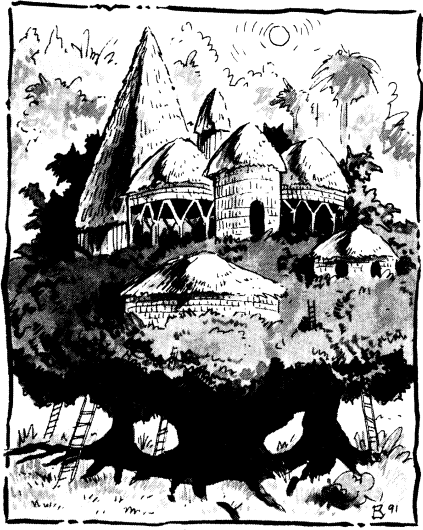
\includegraphics[width=\columnwidth]{images/gulg-1.png}
\end{figure}
\City{Gulg}
{13,500 (80\% humans, 7\% elves, 5\% dwarves, 3\% muls, 2\% half-elves, 2\% thri-kreen, 1\% other).}
{Agafari, copra, feathers, livestock, spices, textiles.}
{Common, Dwarven, Elven, Gulgan.}
{
	The city-state of Gulg sits inside the southern portion of the Crescent Forest, almost directly east of Tyr. Being east of the Windbreak Mountains, Gulg was spared the devastation that the Great Earthquake visited on the cities and villages to the west. That doesn't mean that life in Gulg has remained unaffected by the changes sweeping through the Tablelands. In a few significant ways, Gulg has been changed the most.

	Gulg's sorcerer-queen, Lalali-Puy (LE female champion of Rajaat stage III dragon, defiler 5/telepath 6/arch defiler 5/thrallherd 4/cerebremancer 5/Athasian dragon 2), is the absolute monarch of her realm. Her subjects consider her to be the Oba, the forest goddess. Over the centuries that she's been in power, Lalali-Puy has come to relish the worship and adoration her subjects heap upon her. In fact, though she remembers her origins as a Champion of Rajaat and a sorcerer-queen, she prefers to think of herself as the goddess her people believe her to be.

	To the Oba of Gulg, the abundance of rain---even the violent rain that accompanies a Tyr-storm---is a blessing to Athas. She has proclaimed this blessing to be a gift from the forest goddess. ``No longer will Gulg be solely concerned with the well-being of Gulg,'' the Oba declared to her people. ``Wherever the rain falls, there will the forest grow. And wherever the forest grows, the forest goddess will be there, for all the forests belong to the Oba.''

	Behind the rhetoric, Lalali-Puy actually wants to help restore the vitality of Athas. The Gulgs have always had an enlightened understanding of the interconnected nature of all life, so they've always treated the forest as a precious resource that must be maintained and not depleted. This attitude comes right from the Oba herself, which may seem strange as she is a defiler of extreme power. Since taking over Gulg, however, she has learned to temper her use of defiling magic in favor of keeping her forest healthy.

	Of course, this attitude was one of the contributing factors to the problems with Nibenay. The Nibenese saw the forest as a resource to be exploited, not a living thing that cares for its inhabitants as they care for it. Nonetheless, Lalali-Puy has made the first moves toward a peaceful existence with Nibenay, going so far as to teach the sorcerer-king how to preserve the life-giving environment of the Crescent Forest.

	The Oba's motivation isn't entirely selfless. She believes that when the forests return to Athas she will be deified by all races, just like she's been in Gulg. ``Let Nibenay and Hamanu play as sorcerer-kings,'' she has decided, ``for in the end I will be as a god to all of Athas.''
}
{
	The \emph{dagada} is the single most influential social force on Gulgs outside of the immediate family. The dagada is an extremely close-knit community that shares attributes of both clans and neighborhoods found in other societies. It is similar to a neighborhood in that it is a social organization defined first and foremost by physical proximity. It is like a clan in the role that it plays in acculturating an individual to the values of the society.

	The word dagada is used to describe both a cluster of huts and the people who live there. A dagada can contain up to 100 huts, and typically includes a number of families, though extended families may not necessarily live in the same dagada. Each dagada has a large degree of autonomy in managing its affairs as well as a degree of responsibility for all the members of the dagada. All parents have the burden of raising the young children of the dagada. Elders are responsible for educating the youths as they go. All members have a social duty to care for those who cannot provide for themselves.

	Life has always been more tolerable in Gulg than in any of the other city-states under the rule of sorcerer-kings. In some ways, life has actually gotten better for the Gulgs. The Oba's newfound crusade to restore Athas has made her more forgiving of and generous to her loyal citizens. In the spirit of cooperation, she has selected her best templars to travel the Tyr Region and spread the word of restoration. These templars have a twofold purpose. First, they help show the rest of the Tablelands how to work in harmony with nature, which Lalali-Puy hopes will hasten the reforestation of the world. Second, her templars pass along the tale that the rain is a blessing from the Oba, thereby increasing the number of people who know of and believe in Lalali-Puy.

	Except for the aid these templars have provided to Nibenay, no other city-state has thus far been targeted by the Oba's select force. Instead, the templars visit villages and oasis communities, teaching and preaching as circumstances permit. Some places have welcomed the templars, others have driven them away. Those communities that have actually experienced a Tyr-storm, for example, are quick to attack anyone who claims to be associated with their fearful properties, while those desperately in need of water invite them in.
}
{
\begin{figure*}[b!]
\centering
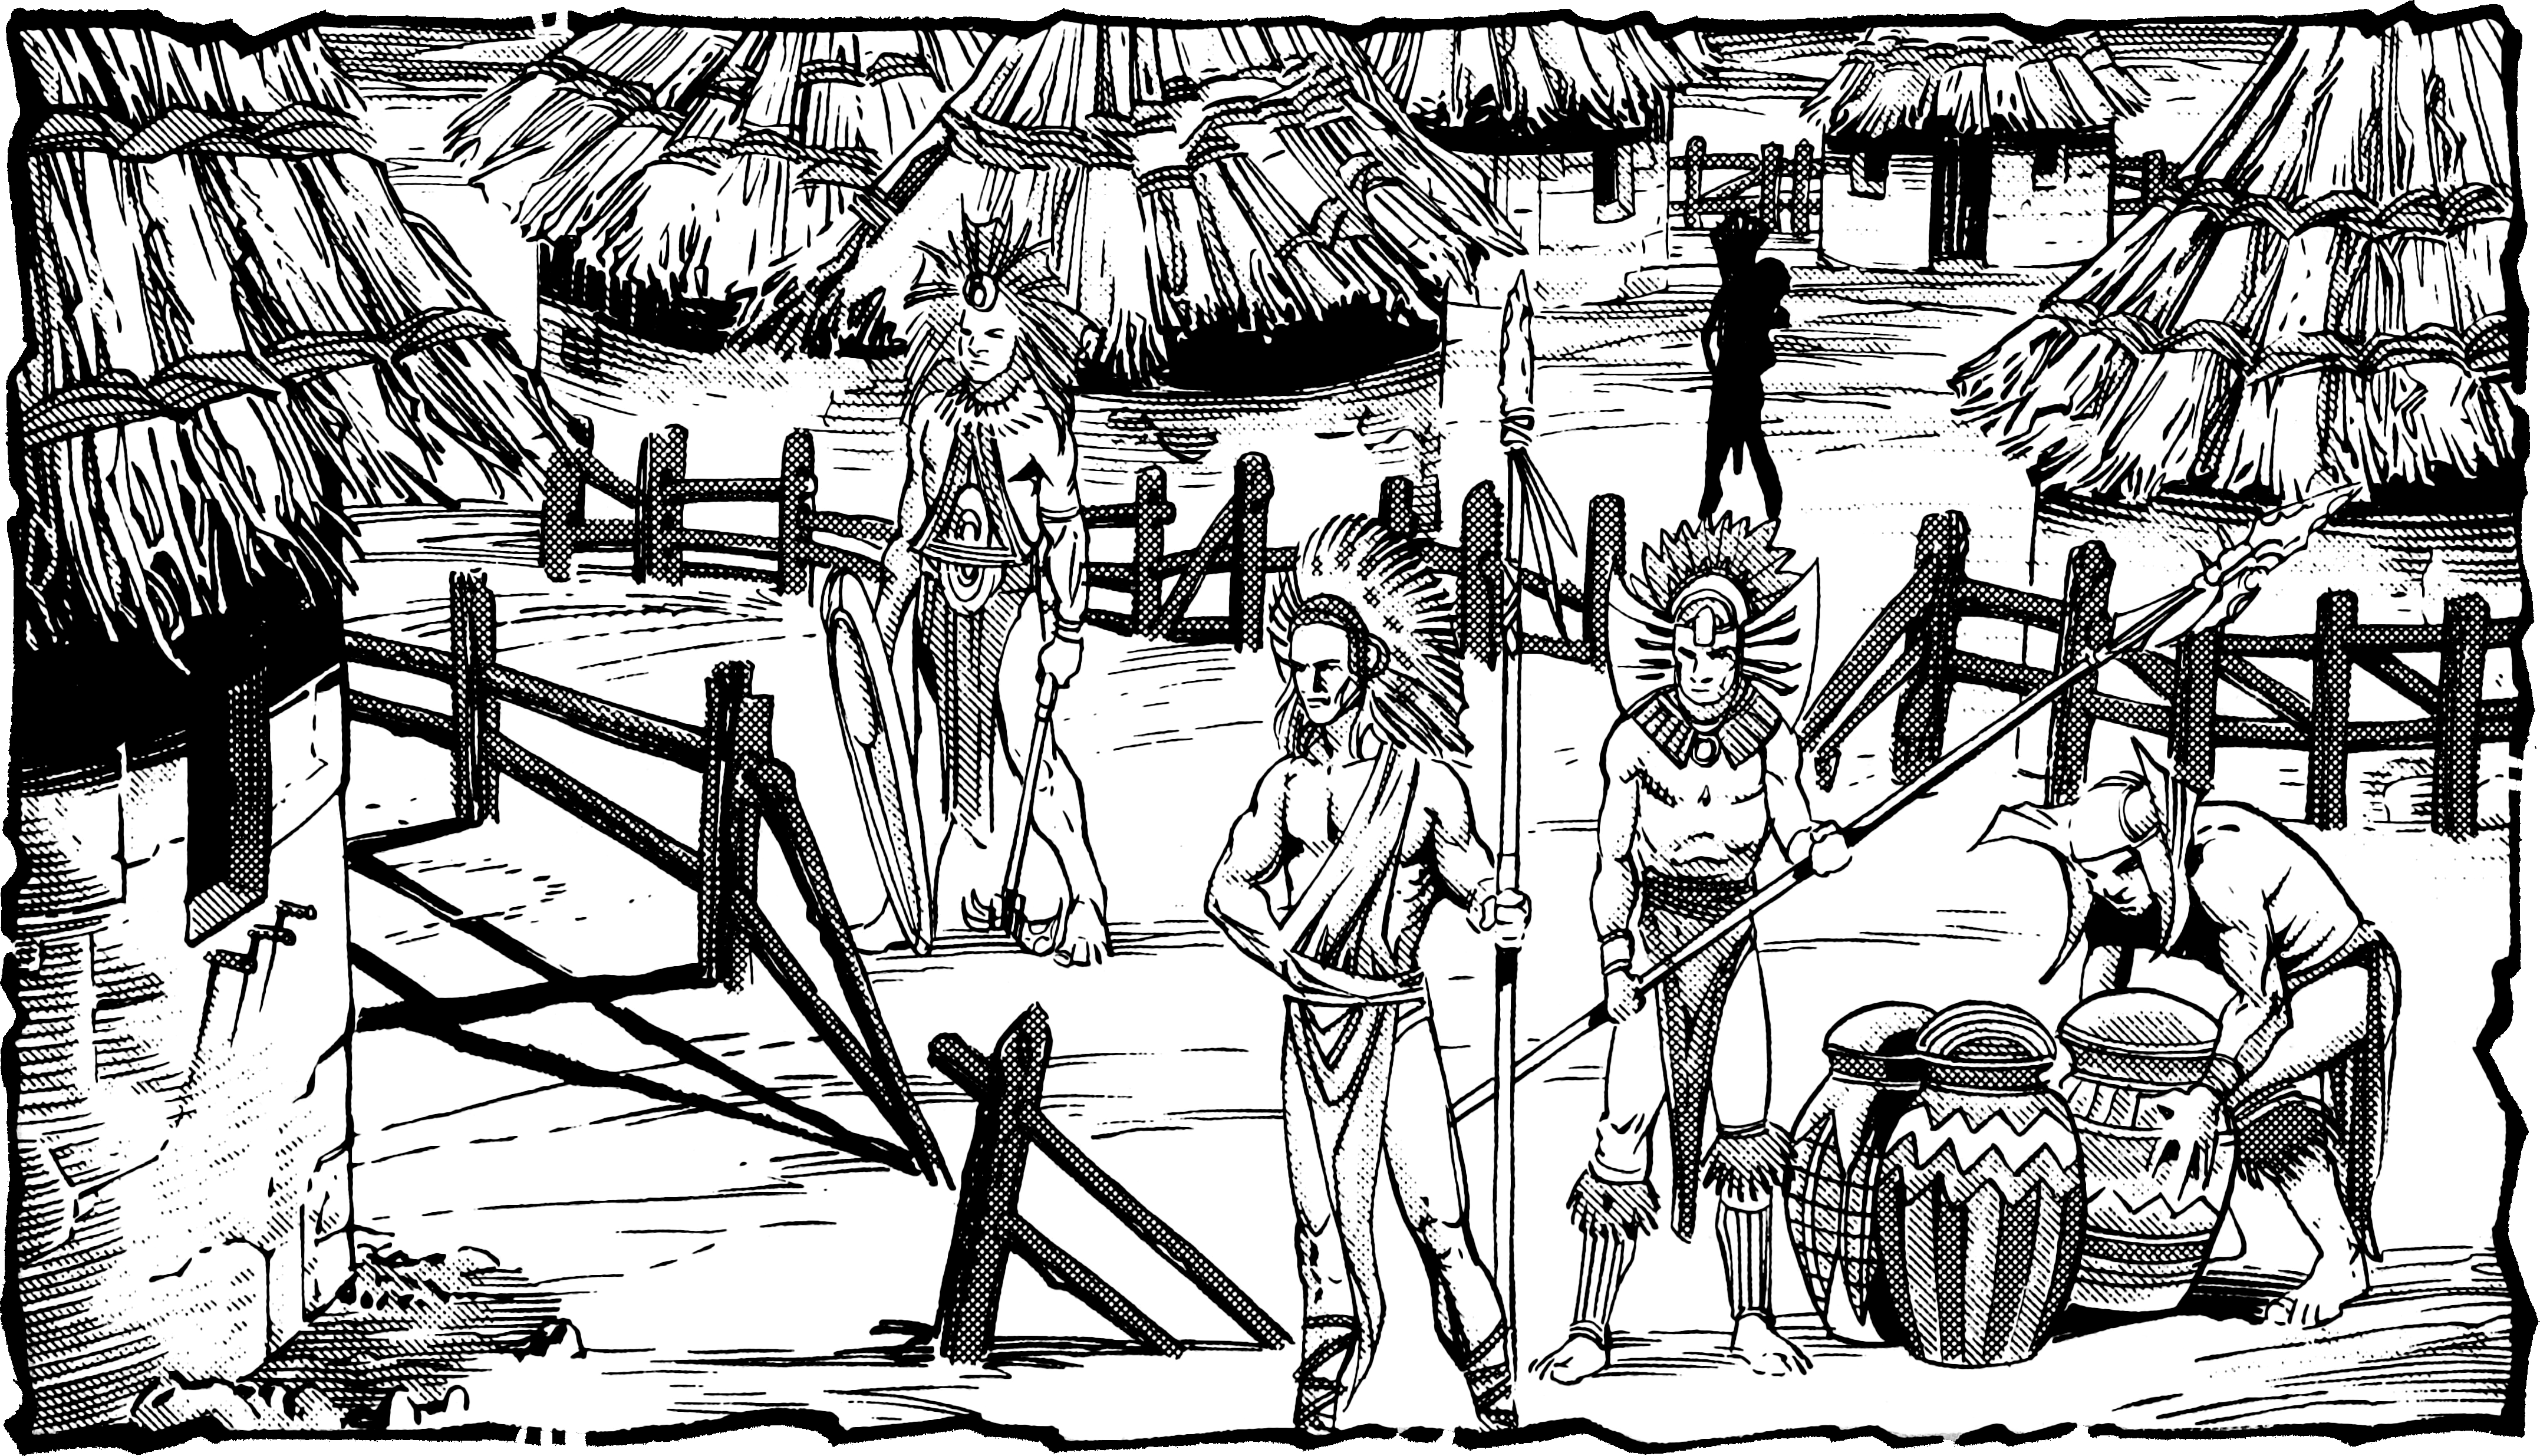
\includegraphics[width=\textwidth]{images/gulg-2.png}
\end{figure*}

	In many respects, Gulg is not like any of the other city-states of the Tyr Region. It's a living city, grown from vines and trees instead of constructed from brick and stone. The outer walls of the city, for example, consist of a thick hedge of thorny trees. The Oba lives in the tallest branches of a huge agafari tree, while her templars inhabit the lower branches. There are no paved or cobblestone roads leading through Gulg. Instead, forest paths and trails wind their way between the trees.

	There have been few major changes in the way Gulg is ruled. The Oba remains the owner of everything, distributing food, water, and other supplies to where they are needed most. Her templars continue to oversee the military, economic, and agricultural aspects of the community on behalf of the forest goddess. Nobility is still an earned position, not one granted by an accident of birth. The nobles hunt the forest for fresh meat, while slaves commanded by the templars gather the wild fruits, nuts, and berries that round out the dietary concerns of the community.
}
{
	\textbf{House Inika}: House Inika, the largest merchant family based in Gulg, is smaller than the typical merchant house. They specialize in small light weight goods of high value, such as spices, gemstones, and feathers from the exotic birds of the Crescent Forest. Inika maintains cordial relations with most of the other houses as it has a reputation for being nonconfrontational. Direct force is rarely used against rivals, with intrigue and economic means being the house's preferred means of strike back at rivals who try to take advantage of the house. The matriarch of the house is Andiama Inika (LN female human, rogue 14/ dune trader 5) who has ruled the house for more than two decades.

	\textbf{Judaga}: Nobility in Gulg is not granted by birth. Instead nobles must earn their position by proving they have the hunting skills necessary to provide meat for the rest of the community. There are several ways in which a citizen can become a noble. One of the most widely known ways a hunter can earn the rank of nobility is by participating in the Red Moon Hunt. During the hunt, prisoners are released unarmed into the Crescent Forest, and a thousand seconds later the hunters are sent after them. If a hunter returns with the head of the prisoners he has earned noble status, which will be bestowed upon him in a ceremony at the next High Sun. The Red Moon hunt is held on nights when the moon Ral is full and alone in the night sky.

	\textbf{The Paper Nest}: The Paper Nest is a secret society comprised of nobles favored by the Oba. The twelve to twenty-four members meet in a secret chamber in the trunk of the Sunlight Home to perform the sacred task of making paper. There is another reason for the group's existence besides making paper. Lalali-Puy attends the meetings and listens as the members debate current problems, offer advice, and present their counsel. At no other time does the autocratic Lalali-Puy allow her subjects to participate in the city's governance.

	\textbf{The Veiled Alliance}: A significant change in Gulg society concerns the Veiled Alliance of the city. Gulg's Veiled Alliance has always actively worked to restore Athas to its verdant glory, never directly opposing the will of the sorcerer-queen.

	Now that the Oba has declared her own intentions for restoring Athas, the two seem to have less to fight over. The Oba has even extended a ``peace leaf'' to the Alliance, calling for the preservers to shed the veil of secrecy and join the forest goddess's quest to save the world. The Alliance hasn't responded yet, but rumors persist that the preservers will soon come out of hiding in the forest city. The Alliance's leader, Aukash-Pad (LG male human, preserver 6/veiled one 5/earth cleric 3/psychic theurge 1), is utterly committed to restoring Athas' life force. If the Oba continues to genuinely work toward that same goal, he may be forced to join with her for the good of the world.
}
{
	\textbf{Losthome (Thorp, 60)}: Losthome is a halfling community deep in the Crescent Forest. The community is less than 10 years old and was formed when the Oba of Gulg attempted to form an alliance with a halfling tribe from the Forest Ridge. An agreement was made, but shortly after the halfling warriors arrived in Gulg, their chief died. The halflings believed that the death of their chief ended the agreement and sought to return to their home, but Lalali-Puy refused to let them go and imprisoned them. Over the years since, most of the halflings have escaped into the Crescent Forest and banded together around their leader, Zivlil (N male halfling, preserver 5/kineticist 3/cerebremancer 2). The halflings maintain no permanent settlement but roam an area of the forest approximately 40 miles wide, in which they have a number of prepared resting areas. The halflings wish to keep their existence a secret to convince the templars of Gulg that they died in the forest. So they kill any nonhalfling who sees them.
}
{
	\textbf{The Drum Circle}: The bard's quarter in Gulg is centered around a dagada called the Drum Circle. The bards of the Gulg specialize in percussion instruments. The most skilled bard in the Drum Circle is considered to be Ken-kenku Vek (NE male half-elf, bard 12). His skills as a drummer and an assassin are legendary.

	\textbf{The Forest Arena}: The gladiator arena of Gulg is located outside the city's mopti wall in the Crescent Forest. Trees and vines intertwine with the arena to give it the appearance of growing from the forest. The floor of the arena is oval shaped, and covered with grass. A number of trees grow from the arena floor; however, none is closer than 6 meters from the arena's walls, to prevent gladiators from using them to escape.

	\textbf{The Grove of Mysteries}: Throughout the forest surrounding Gulg there are a number of forest groves called the Queen's Groves. Entrance into one of these groves without the permission of the Oba is punishable by death. The Grove of Mysteries is the largest of the Queen's Groves and is tended by the druid Extambolan (N male mul, druid 5/grove master 10).

	\textbf{Mopti Wall}: Unlike the walls of other city-states, the walls around Gulg are alive. The Mopti wall is a miles long thorn wall make of thickly packed brambleweed that surrounds the city.

	\textbf{The Seers' Dagada}: When a Gulg shows psionic potential they are sent to the Seers' dagada, where they receive instruction from experienced psions. The teachers are patient and encouraging towards the students. Even those who fail to develop enough psionic potential are not cast out, but remain part of the Seers' dagada performing physical chores for the other members.

	\textbf{Sunlight Home}: Sunlight Home is the name given to the palace of Sorcerer-Queen, Lalali-Puy. Located in the tallest branches of a massive agafari tree, Sunlight Home towers over the rest of the city. Lalali-Puy's palace is rumored to contain dungeons and secret passages that have been carved into the trunk of the massive tree.
}
{
	\item Ngeli is a small boy of ten years old. While gathering cloves in the forest he was attacked and dragged off by a sloth. His parents are distraught and want to see a rescue attempt made to recover their boy, but the ambo of their dagada ruled that the boy was taken by the nature spirits and should be given up to his fate. Ngeli's parents turn to outsiders, the PCs, to secretly bring back their boy.
	\item The berry harvest has finished for the year. The berries had a strange brownish tint, but seemed fine to the taste. But those who have eaten too much of the berries have been having strange reactions. Some exhibit strange new psionic powers, others become sick and die, and some fall into a suggestive state and will do nothing but what others tell them to do.
	\item Alexia Vordon trades for spices with Gulg. She feels that her house trades at a disadvantage by being forced to deal with the templars. If she can make contact with a member of the spice gathers she is convinced that she will have a better understanding of how good the year's harvest has been and be in a better position to negotiate with the templars. Alexia hires the PCs to sneak her into the city and help her try to befriend someone from the spice gatherers dagada.
	\item Rumors in the neighborhood have begun that a teenage girl is really a witch. The wild rumors began when the girl started wearing a veil that covers her face leaving only her eyes showing. Many hot-headed, superstitious members of her dagada are contemplating drastic actions against the girl. The PCs will have to find some way to stop these rumors. The truth is that the girl has experienced her first heavy case of acne. Unsure of what is really happening to her, and fearful that others will reject her because of her affliction, she hides behind the veil, refusing to remove the veil and revealing her affliction to anyone.
	\item The PCs are invited on a hunt with a group of nobles from Gulg. The nobles seek to test the PCs hunting skills. They hang back letting the PCs take the lead, while hunting a dangerous beast, such as a klar.
	\item The templar, Kampala, has a feylaar as his fetish. When visiting a small client village, he summons the totem spirit, only to have it break from his control and go on a rampage.
}
\City{Nibenay}
{24,000 (60\% humans, 12\% half-giants, 10\% dwarves, 10\% elves, 4\% half-elves, 3\% muls, 1\% other).}
{Rice, timber, hardwood, weapons, copper.}
{Common, Dwarven, Elven, Nibenese.}
{
	Nibenay has been affected by the monumental happenings of recent months, for the Shadow King has changed his approach to ruling the masses and dealing with the neighboring city-states. Like Hamanu and Lalali-Puy, Nibenay (who shares the same name as his domain) witnessed the deaths of the Dragon and the other sorcerer-kings.

	He saw Rajaat reach out from beyond the veil of Athas to wreak vengeance against those who betrayed him. He also saw Rajaat defeated by the efforts of lowly mortals from the city of Tyr. In the wake of these signs and portents, Nibenay realized it was time to reconsider how best to rule his city, for the time for change had come.

	The city-state of Nibenay is located east of Tyr at the northern tip of the Crescent Forest. It barely felt the effects of the Great Earthquake, as it was protected by the Windbreak Mountains. Nibenay has also thus far been spared from Tyr-storms and the growing unrest spreading throughout the Tablelands. If the Shadow King has his way, none of these problems will ever reach his domain.
}
{
\Figure{b}{images/nibenay-1.png}

	Though there have been no major changes to life in Nibenay, enough strange occurrences have been worked into the routine to put a different spin on the city-state. For example, average citizens and even powerful nobles never expected to see the Shadow King, let alone attend one of his courts. Now the Shadow King regularly makes public appearances and shows an active concern for his community. This doesn't mean that life is any harder or easier than it's always been. It's just different. If a citizen or visitor breaks a law and can't afford to bribe a templar, then that citizen or visitor is still going to end up in Nibenay's slave pens.

	The other major change is the city's outlook on matters of a martial nature. The Shadow King and his templars seem to be concentrating much of their efforts on bolstering Nibenay's military might. The army regularly practices in the arena and patrols of the surrounding countryside have increased dramatically. In addition, free citizens and nobles have been ordered to serve in Nibenay's defense. Templars are busy organizing them into part-time militias and regimenting training sessions.

	What the Shadow King is truly concerned about, besides the unrest and upheaval that seems to be spreading throughout the Tablelands, are the rumors claiming that Dregoth has returned. Nibenay knows how powerful the sorcerer-king of Giustenal was. Dregoth was second only to Borys the Dragon in power. If Dregoth and his city have somehow come back from the dead, Nibenay wants to be prepared.

	After all, Nibenay's city-state is one of the closest to the ruins of ancient Giustenal, and he has no intention of losing his domain to a rival that was destroyed two millennia ago.
}
{
\Figure*{b}{images/nibenay-2.png}

	The sorcerer-king Nibenay (LE male champion of Rajaat stage IV dragon, defiler 5/seer 5/loremaster 10/cerebremancer 10/Athasian dragon 2) used to stay behind the scenes. He was called the Shadow King because he rarely left Naggaramakam, his walled sub-city. His templars, who are all female, ran the city with skill and great care. Now, however, the Shadow King has become more prominent.

	In the past, the average free citizen could hope to see King Nibenay once or perhaps twice in an entire lifetime. Since the time of the Great Earthquake, Nibenay has taken a more active role. He still allows his templars to deal with the daily business of government, but now Nibenay has turned his attention away from the mysterious scholarly pursuits that once occupied his time to hold court for the city's nobles and free citizens.

	Nibenay's military might was never a question, but it also was never a major concern of the Shadow King. Now he actively seeks to understand his forces and looks for ways to improve their might and readiness. While the city used to appear to be secure in its own position, it now seems to be gearing up to battle an enemy that only the Shadow King knows about. The problem is that the enemy is change, and no army that Nibenay raises will be able to stop its relentless tide.

	In the wake of all this upheaval, Nibenay's nobles continue to care for and maintain the bubbling springs that surround the city. They don't know what to make of the Shadow King's sudden interest in the business of the city, but many of them are seeking ways to improve their own positions by getting closer to their once-elusive king.
}
{
	\textbf{Poortool's Horde:} Lead by the half-Elven preserver Poortool (LN male half-elf preserver 5/seer 3/cerebremancer 5), the Horde is a raiding tribe to the east of Nibenay. Poortool is a renegade from the Veiled Alliance who seeks to study magic without any restriction that the Veiled Alliance or sorcerer-king Nibenay may apply. He has created a community for likeminded preservers in a village in the foothills of the Black Spine Mountains. He has also allied with the gith of the Black Spine Mountains who provide guards and raiders for his tribe. Poortool seeks to make it difficult for members of the Veiled Alliance in Nibenay to convince its members to leave the Alliance and join him.

	\textbf{House Shom:} House Shom is thought to be the oldest merchant house operating in the Tyr region. For centuries the house amassed great wealth through aggressive trading. However, now the House is seen as passive and decadent. The Shom family members are almost never seen in public and have little to do with the daily business of the house. Instead the family members live decadent lives in their palaces, engaging in expensive parties and balls. The running of the trading house is left to the house agents. Most of the agents place their interests ahead of House Shom's interests, and there is much infighting between agents. This has lead to a decline in the House's prospects over the past few decades. Only the house's immense wealth has saved it from collapse already. House Shom is known to use non-human guards on its caravans and as raiders against other merchant houses, including thri-kreen packs and belgoi tribes. The house is currently ruled by Temmnya Shom (NE female human, defiler 15). Her younger brother, Jebea Shom (LN male human, rogue 3/fighter 2/dune trader 1) has begun a reform movement to straighten out the family's problems, but his popularity threatens Temmnya's position. She has contemplated disposing of him if she can do so without her involvement being discovered by other family members.

	\textbf{Sky Singers:} The Sky Singers elf tribe maintains a permanent market in the Hill District of Nibenay. It is the only known instance of a permanent Elven market. The market is filled with goods of all kinds from the rare to the common. The Sky Singers have a reputation of offering quality products that were not stolen from their previous owners, unlike most Elven tribes. While the tribe numbers over 3,000 members, much of the time the elves are off wandering, leaving only a dozen or so elves to tend the marketplace. But when the tribe returns, the Sky Singers' market takes on a festive atmosphere.

	\textbf{The Veiled Alliance:} Nibenay's Alliance has an utter hatred of defilers. This has led to a rare commodity beneath Athas' crimson sun-idealism. With the help of an ancient spiritual force known as the zwuun, which resides in the hot springs outside the city, the Alliance does what it can to protect wizards who use preserving magic. The Alliance doesn't feel it can oppose the Shadow King directly, so it directs its activities against lesser defilers. Thagya Phon (LN male human, preserver 7/veiled one 10) leads the Nibenese Alliance, though his health has begun to fail him in recent years. He has two goals he wishes to accomplish before he dies: He longs to discover what Nibenay's scholar slaves have been working on in the Naggaramakam, and he has a dream of mounting the Shadow King's head on the obsidian pedestal that rises from the floor of his spartan quarters.
}
{
	\textbf{Cromlin (Hamlet, 150):} The trading village of Cromlin sits on the shores of the Silt Sea, northeast of Nibenay. House Shom runs the village, though House M'ke has a sizable operation as well. Together they handle the vast majority of trade from the north, as traders attempt to bypass the chaos of Raam. Cromlin traders use silt skimmers to navigate the silt shoals, keeping the trade route to Break Shore open. The shoal navigators of Cromlin are in high demand, for they are among the select few who can lead silt skimmers along the buried paths.

	Cromlin is a wild place, full of people who are too untamable to live in the cities. Thieves of all sorts reside in the village. Silt pirates use it as a haven and other scoundrels and restless souls are drawn to its sandy shores. Master trader Hurdll Crost (N male human, bard 10/dune trader 5) and his agents turn a blind eye towards shady characters as long as they remain to do business in his village.

	\textbf{Salt View (Small Village, 550):} Nestled in the Mekillot Mountains, Salt View is a chaotic sprawl of tents and buildings located within a large cavern on the mountain's eastern face. Ex-slaves of all races fill the community. The tribe originally practiced raiding as its primary occupation, but today it is known for a lavish form of storytelling called theater. Salt View's traveling theater troupes are welcome across the Tyr Region, though they present themselves as free merchants from the independent House Fyra (a cover for Salt View activities). The troupes perform for caravans, at oasis villages, and even in the city-states of Tyr, Nibenay, and Balic.

	\textbf{Vavrek (Thorp, 200):} Vavrek is typical of the small farming villages located throughout the Fertile Crescent. The village is located southwest of Nibenay within sight of the Crescent Forest. The villagers grow vegetables, mostly soybeans. The land the village is built on is owned by the Koelse noble family, to which the villagers must pay rent. The village is administered by a templar-wife of Nibenay named Sonyalah (NE female human, templar 5/wife of Nibenay 3).
}
{
	\textbf{The City Reservoir:} The Shadow King had this enormous stone cistern constructed centuries ago to supply the city with water in the event of a siege. The top of the reservoir is covered and a lush garden, maintained by the templars, grows on top of the reservoir.

	\textbf{The Coliseum:} The coliseum rises above the dilapidated buildings in a rundown part of the city. The size of the arena is immense, taking up four city blocks and rising six stories high. It is an ancient building and it is said that not even the Shadow King knows when the coliseum was built and by whom. Elaborate carvings and etchings cover the coliseum's stonework. The square shaped arena floor stretches almost a quarter of a mile across.

	\textbf{Monasteries of the Exalted Path and of the Serene Bliss:} Nibenay has a tradition of monasteries. The two orders are called the Exalted Path and the Serene Bliss. The monks pledge loyalty to the King and their teachings include the quiet acceptance of authority, so the templars tolerate them. They are treated with great respect by the citizens. The monks live very aesthetic lives, tending gardens and mediating. Many of the monks, especially those of the Exalted Path, study psionics. The Exalted Path consists entirely of male monks and is led by Thong Nal, (CN male human, air cleric 3) who encourages the study of psionics at his monastery. Other monks become artisans who specialize in the carving of the images that cover the buildings of Nibenay. The Serene Bliss is an all female order and is led by the abbess Au Treng (LN female human, cleric 4).

	\textbf{Naggaramakam:} The Naggaramakam is a walled forbidden inner city where the sorcerer-king Nibenay lives with his templar-wives. Only templars are permitted to enter and leave the Naggaramakam. While slaves are permitted to be brought into the Naggaramakam, once inside they are never allowed to leave. No free citizen is ever allowed to see the inside of the Naggaramakam. The sorcerer-king's palace is said to be carved into a stone relief of the Shadow King with dancing women, representing his templar-wives, strung together as if they were his hair.

	\textbf{The Omnipotent Receivers:} A line of large statues of sorcerer-king Nibenay stand on each side of the main road leading to the city. The statues are called the Omnipotent Receivers as it is believed that King Nibenay sees all that the statues see.

	\textbf{The Plain of Burning Water:} The city of Nibenay is situated on the border of a large area of hot springs. Called the Plain of Burning Water, the hot springs provide the water needed by the citizens of Nibenay. Each noble house owns at least one of the hot springs which is the source of much of the wealth of the nobility.

	\textbf{Sage's Square:} Sage's Square is the largest open area inside of the city. The grand emporiums of all the dynastic merchant houses are located around the square and are the center of trade in Nibenay, where almost anything can be purchased. The square was named Sage's Square because scholars and sages use to gather under the shadow of the huge agafari trees that grew in the square, and debate philosophy. This tradition ended only a few years ago when a renegade defiler, fleeing the templars defiled the trees. King Nibenay had the dead trees removed from the square, and ordered that no other trees be planted in the square as a public reminder of the danger of renegade defilers.

	\textbf{The School of Augurs:} The school of Augurs is the largest school for psionic instruction in Nibenay. The head master is a dwarf named Djef, who developed a scheme to help support the school by hiring out its students to transfer telepathic messages and to teleport-deliver small parcels.
}
{
	\item A disguised dray agent has entered Nibenay seeking to make contact with nobles disgruntled with the Shadow-King's rule. The dray tries to gather together as many nobles as possible so that when Dregoth makes his attack on Raam, he can start a rebellion in Nibenay to distract the Shadow-King from interfering in Dregoth's plan.
	\item The templars attempt to ambush a cell leader of the Veiled Alliance who they believe is staying at the same inn as the PCs. During the templar raid, one of the PCs is mistakenly identified as the Veiled Alliance member. Capture means execution, so the PCs must flee. If the PC makes it out of the city, his problems are not over. Because of the secrecy of the Veiled Alliance, the subordinates of the cell leader have never met him before. When the templars identify the PC as the cell leader, the other members assume it to be true. When the PC flees the city the cell members attempt to enforce Requital, believing the PC has tried to resign from the Veiled Alliance.
	\item Ramai is a templar of Nibenay, who is responsible for interrogations. Dedicated and highly skilled in all manner of interrogation and torture techniques, she holds some respect within the templar hierarchy. Her career appeared promising until one day, inexplicably, Ramai fell in love with one of her victims, a young man named Tongkol. Unable to bear the thought of Tongkol suffering under torture but also realistic enough to know they can never be together, she assigns the PCs the task of spiriting Tongkol out of the city. Ramai will not offer the PCs any direct help, but can give them information to help them succeed. If the PCs fail and are captured, Ramai will deny any involvement with the PCs and see that they are executed quickly to silence them.
	\item Gith raiders have discovered a previously unknown ancient catacomb that allows them to enter the city undetected. They raid some dwellings in the city and attempt to flee back the way they came. But undead that were angered by the gith's trespass have arisen and prevented the gith from getting out of the catacombs. The PCs are sent into the catacombs after the gith and must also face the undead horrors.
	\item One of House Shom's merchant forts has been overrun by gith. The PCs are hired to lead the assault to retake the desert fortress.
	\item A preserver of the Veiled Alliance asked the zwuun for help on his latest research. The zwunn's answer directed the preserver to the site of ancient ruins that overlook the road to North Ledopolus where he could find what he sought. Unsure if the zwuun was being mischievous or not, the preserver sends the PCs to scout out the ruins.
}
\begin{figure}[b!]
\centering
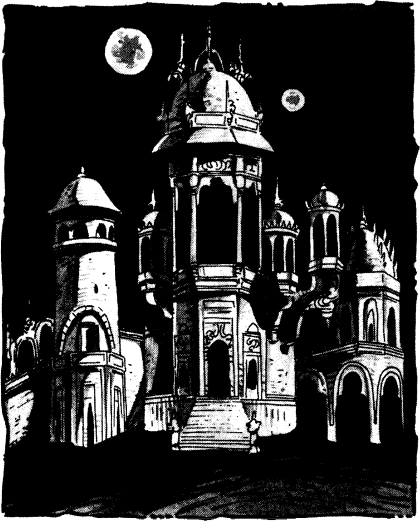
\includegraphics[width=\columnwidth]{images/raam-1.png}
\end{figure}

\City{Raam}
{40,000 (40\% humans, 20\% dwarves, 15\% elves, 10\% muls, 5\% half-elves, 5\% half-giants, 4\% thri-kreen, 1\% other).}
{Silver, gems, flint, jute, silk, textiles.}
{Common, Dwarven, Elven, Raamite.}
{
	Shortly before the day of the Great Earthquake, the sorcerer-queen Abalach-Re was killed in battle with Sadira of Tyr. When the news reached Raam, it was the spark that ignited the fires of anarchy, and now Raam burns. But Raam was a city on the brink of revolution even before the death of its queen. Since Abalach-Re's death, the city has collapsed into chaos. Various factions have grabbed whatever power they could, and Raam teeters on the brink of civil war.
}
{
	Raamish society revolves around a caste system. Each citizen is born into a caste and can never leave it. Members of one caste cannot marry or associate with others from another caste without becoming unclean. Caste and race are not related, and a member of each race can be of any caste.

	The highest caste is made up of priests. This caste includes clerics and druids, as well as teachers, scholars and wise men. Members of this caste wear white garments to distinguish themselves.

	Below the highest caste, is the vizier caste. The templars and soldiers of Abalach-Re fall into this caste. The members of the vizier caste typically wear silk clothing dyed a variety of colors.

	The next caste includes the majority of the nobles of Raam, as well as artisans, and tradesmen. Wealth has no affect on one's caste. The richest tradesmen will never rise above his caste. This caste typically dresses in clothing made of less expensive material than the silk worn by the vizier class.

	The laborers caste is the largest caste and the lowest. It includes all servants and unskilled workers as well as the vast numbers of slaves. Laborer caste members wear simple white linen clothing.

	Below the laborers caste are the truly desperate. Outcastes are those who most handle dead animals and people. Butchers, morticians, and tanners are all included in this caste. They are considered so unclean that they must live outside the city to prevent them from polluting the rest of the citizens.

	The environmental disasters of recent months have had very little impact on Raam. The Great Earthquake was barely perceived, for it caused little damage and no deaths. No Tyr-storm has yet visited the city-state, so Raam's residents have yet to experience the devastation that such a storm can inflict. The death of Abalach-Re and the resulting struggle for power, however, have caused more death and destruction than any force of nature.

	Raam has been divided into armed camps controlled by greedy, power-hungry warlords. Some call themselves templars, others nobles, liberators, or merchant lords. All are raiders and bullies, seeking to use strength as a means of control.

	These armed camps don't even make a pretense of peaceful coexistence. Skirmishes over disputed territories are constantly being fought, as are battles over caches of weapons or supplies-even just to determine which side is stronger! It won't be long before all-out war breaks out to see if one leader and his faction can conquer the others and restore order of some sort to the city. This war, of course, may simply wind up destroying Raam and reducing the verdant belt it occupies to a wasteland.

	Understandably, the free citizens live in a constant state of fear. They have nowhere to go, nowhere to turn to, and conditions within the city become more terrible every day. Some citizens have appealed to one faction or another, offering to become indentured slaves for the protection and sustenance offered by the vying warlords.

	Every day, more and more citizens surrender their freedom in exchange for a safe place to sleep, a cool drink of water, and a bit of food to fill an aching stomach.

	The slaves of the city have fared even worse than the free citizens. Their masters have been replaced by heartless owners who treat the slaves no better than living tools that can be replaced when they break. Some slaves, embracing the legends of Rikus, Neeva, and Sadira of Tyr, have rebelled, using the opportunity presented by the chaos. One group has come under the leadership of a gladiator named Korno (CN male mul, barbarian 1/gladiator 4/arena champion 4). Between Korno's military daring and expertise and the cache of weapons his followers found in one of Abalach-Re's many hidden treasuries, this group of slaves has set itself up as another armed band in a city of gangs. Korno has called for all slaves to join his community, for when they have the numbers to go along with their dreams they will rise up and overthrow all their masters. Korno, however, is as cruel and ruthless as any of the other leaders of the armed bands. The slaves that have flocked to his side continue to be treated as slaves, working to make life easier for Korno and his best warriors.

	With food and water in short supply and violence rampant in the streets, it is little wonder that the people of Raam are turning to anyone or anything that claims to have a solution. In this volatile environment, revolution seems to be inevitable. What the outcome of such an event will be is unknown, but by all indications it will be bloody in the extreme.
}
{
\begin{figure*}[b!]
\centering
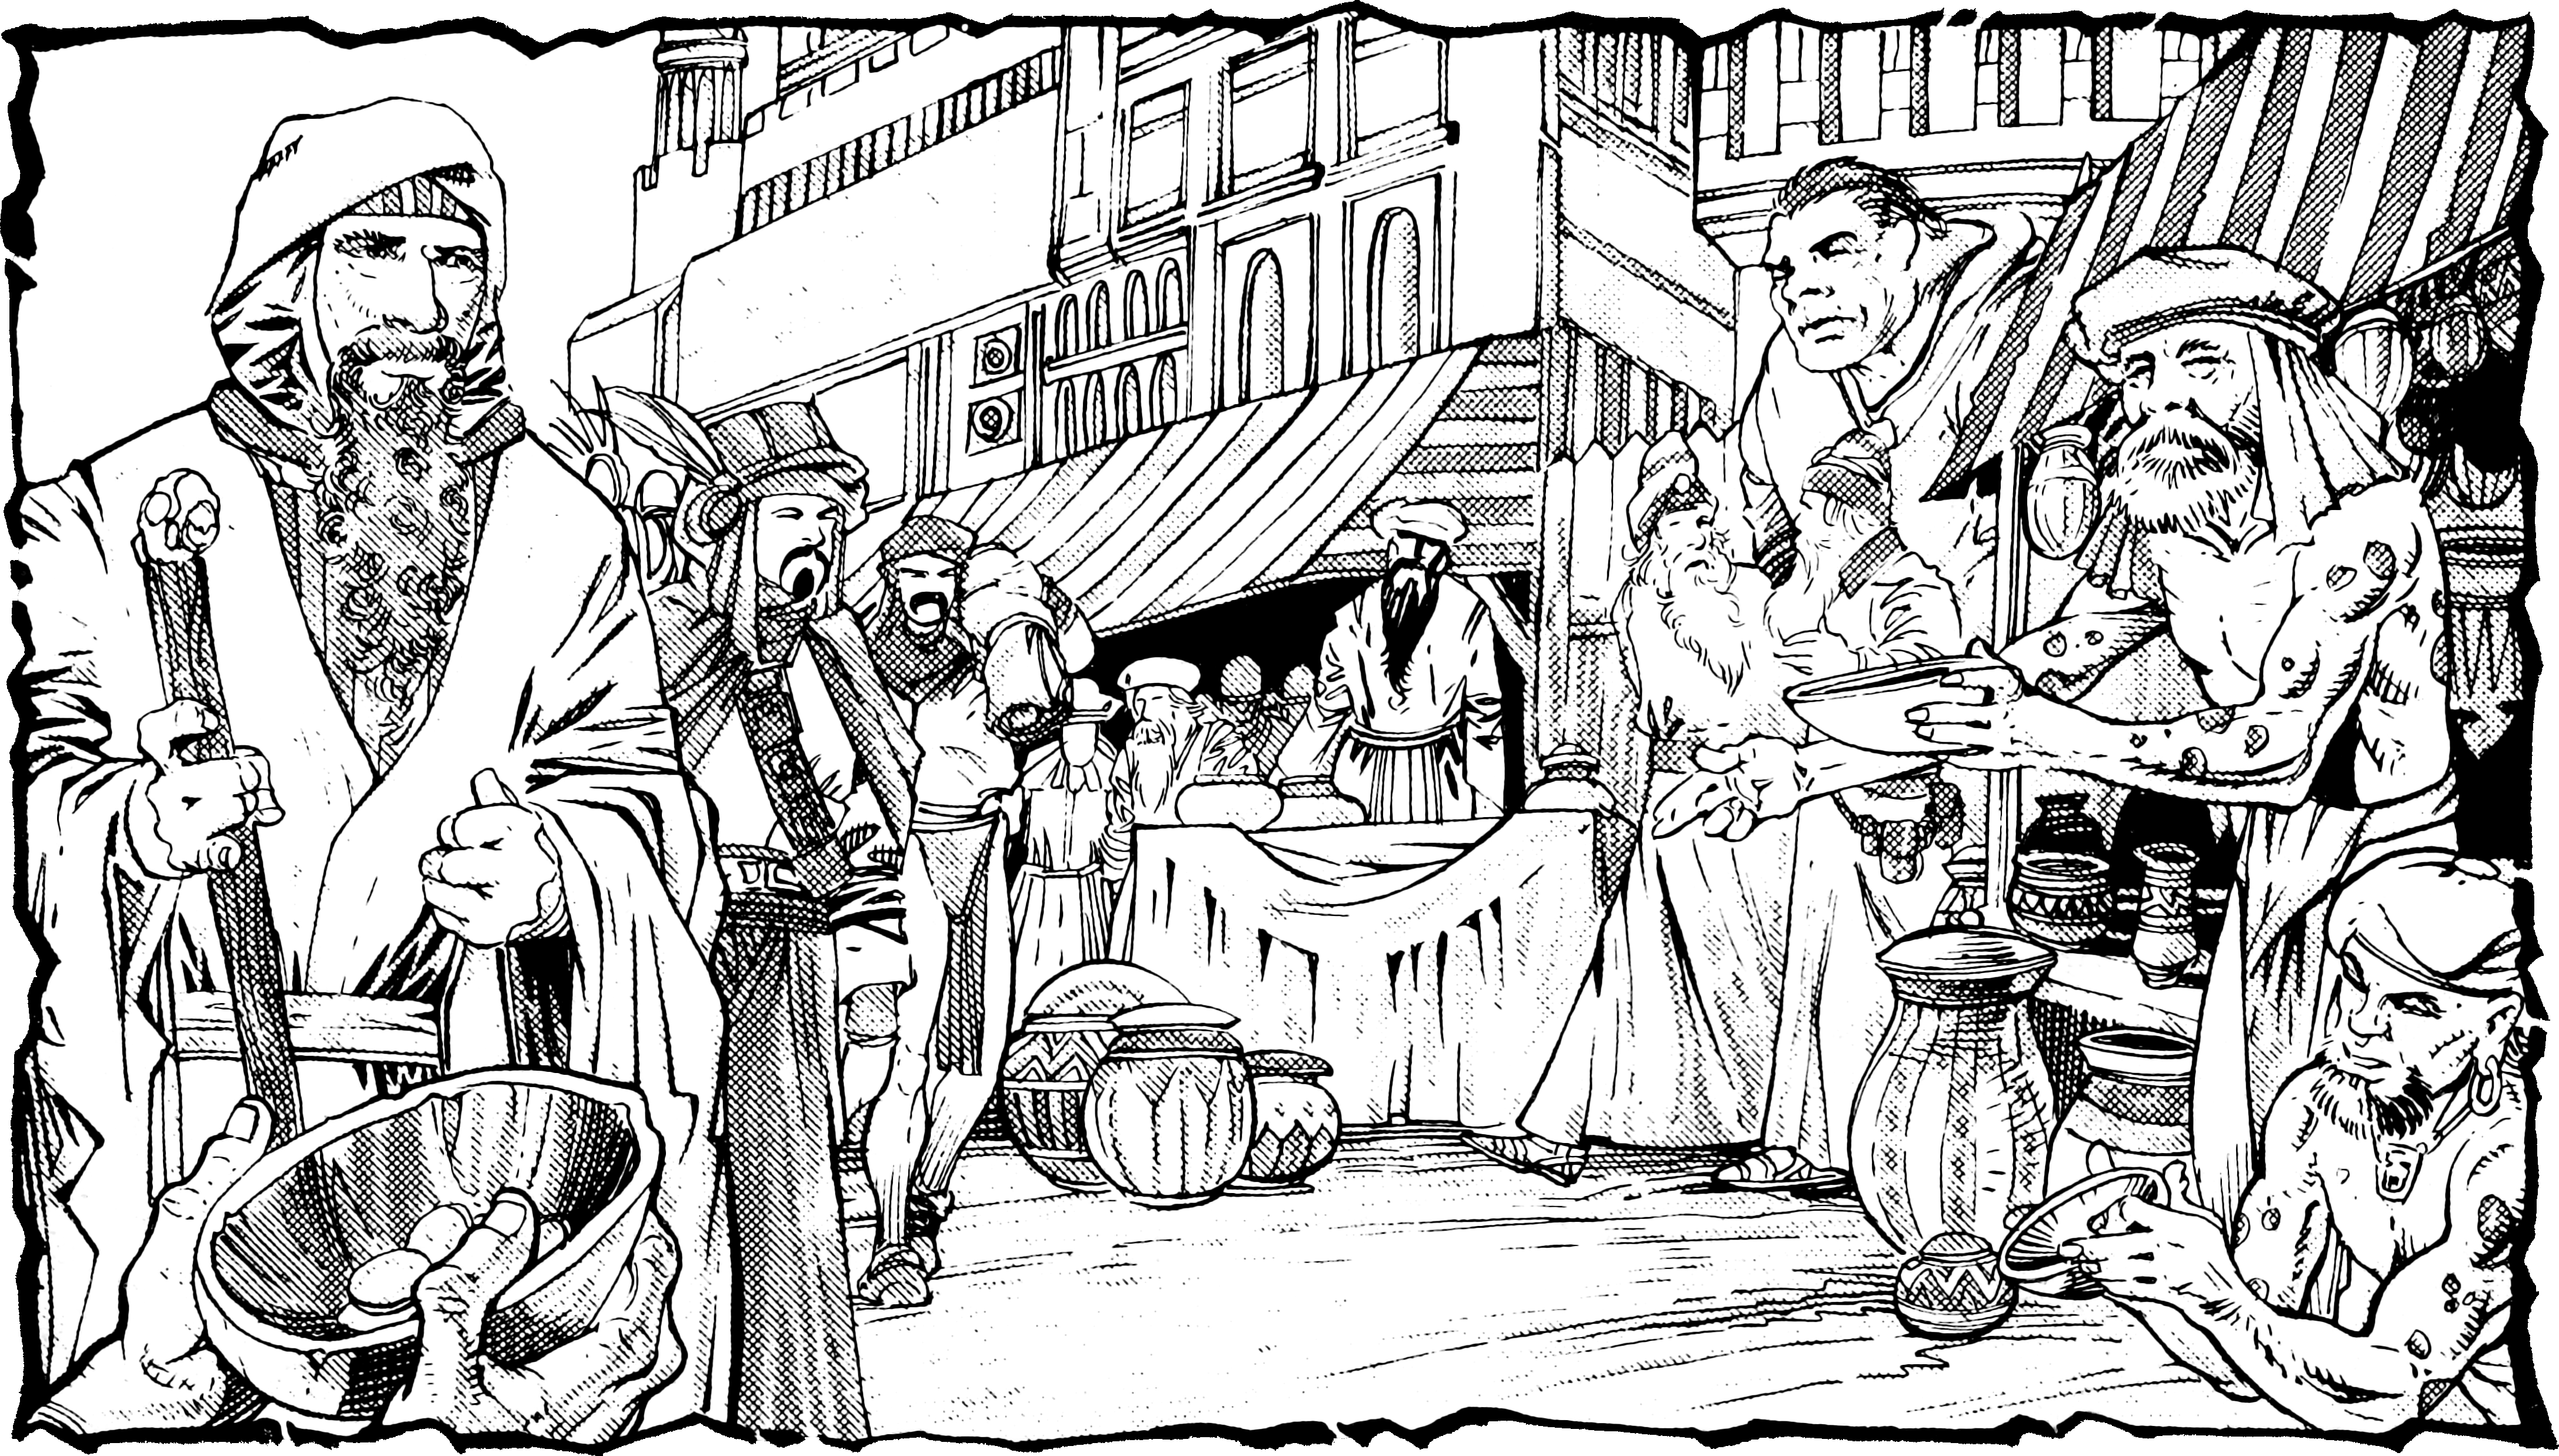
\includegraphics[width=\textwidth]{images/raam-2.png}
\end{figure*}

	The government of Raam still exists, but it has almost no power in the face of the violence and chaos ravaging the city. The templars who haven't fled in fear or tried to hide among the populace as regular citizens continue to administer the city, but it is clear the city no longer functions the way it used to. These templars have only their bureaucratic skills to fall back on, as their ability to use priestly spells vanished with Abalach-Re's demise. The templars continue to call for the worship of Badna, the mysterious (and imaginary) being the sorcerer-queen claimed to receive her powers from. Most people ignore these calls to worship, for they never believed in Badna anyway.
}
{
	\textbf{Leviath the Calm}: Leviath the Calm (LN male half-giant, shaper 9) is an unusual half-giant who speaks of peace and tranquility to all who would listen. His words are spoken with kindness and sincerity, and have had a profound effect on the masses, among which he has developed a large following. Despite his large size and strength Leviath is said to have never raised his voice in anger or struck a blow to harm another living creature.

	\textbf{House M'ke}: The merchant houses have taken one of two tacks regarding conducting business in Raam. The first option, chosen by the vast majority of merchant houses, was to get out of town and take their business elsewhere. The second option, embraced by House M'ke as a prudent enterprise that will ensure its own survival, was to seize control of as much of the city as possible. House M'ke and its army of mercenaries now control most of the merchant district. Armed bands wearing House M'ke's colors periodically sweep through the city, looting and pillaging until they gather enough goods to fill a caravan. This caravan then sets out across the Tablelands to conduct trade as any merchant house caravan would. Only in Raam does House M'ke behave like a conquering army of raiders-because in Raam, that's what House M'ke has become. A few of the more daring (or desperate) merchant houses return to Raam from time to time to test the climate, but they usually wind up losing their goods to one or more of the armed camps seeking dominance in the city.

	\textbf{Night Runners}: The strangest group to stake a claim in Raam's power vacuum is the elf tribe known as the Night Runners. Prior to Abalach-Re's death, the Night Runners maintained a small presence in Raam. Now this group of elves-which specializes in the ``shadow arts'' of espionage, assassination, and extortion-has decided to take a more active role in Raam society. A large portion of the elf quarter and the tradesmen's district has been taken over by the Night Runners. Besides holding and expanding their own territory, the Night Runners continue to sell their unique services to those who can afford them---including noble houses, merchant camps, and even templar domains. In the end, the Night Runners plan to control the entire city, making it the first elf city in thousands of years. Until then, the elves don't mind working for the bands they're competing with, for it gives them an easy way to keep tabs on how the factions are doing.

	\textbf{Nobles}: One of the largest groups claiming dominion over sections of Raam is the noble families. Like the raiding tribes of the sandy wastes, the nobles pillage and plunder for the things they want and need to survive. The nobles have expanded their areas of control. While each family started with a small piece of land and the road adjoining it, those with the power and audacity to press their advantage have grabbed whatever they could hold onto. Like the raiding tribes, the noble camps are savage, ruthless, and have only their own interests at heart.

	\textbf{Prophets of Dregoth}: Strange figures with bizarre accents who hide their features beneath many folds of robes preach of Dregoth the Savior. These prophets claim Dregoth is a god who will bring salvation to Raam if they lay down their weapons and accept him.

	\textbf{Templars}: The main body of templars occupies one camp, centered in the templar quarter of the city. Various rogue templars command smaller parts of Raam, claiming from as little as one building to as many as several blocks as their personal domains. They defend these domains with troops that were once loyal to Abalach-Re but now follow their templar commanders.

	Under Abalach-Re's reign there were two organizations of templars assigned to police the city. The mansabdars were the public force. They were assigned to guard and patrol duties. Though the larger of the two police forces, the mansabdars were corrupt and many were incompetent. The kuotagha was the secret police force. These ruthless enforcers were tasked with administering justice as they saw fit. Disguised as merchants and artisans, they moved freely among the population spying out sedition and unlawful behavior. When they judged someone guilty, the kuotagha executed the suspect without trial, immediately and by surprise. All kuotagha members carried a special garrote called a ghi, for use in such situations.

	\textbf{The Veiled Alliance}: The turbulent conditions in Raam haven't made it any easier for the city's Veiled Alliance. The preservers continue to operate in secret, but the contacts they once had in all levels of government have been lost. Nanda Shatri (LG female human, preserver 7/telepath 4/veiled one 10) continues to lead the Alliance and still seeks to become an avangion so that she can help restore Athas' lost vigor. However, beyond the vague rumors that Urik's Alliance had created such a being some years back, Shatri is no closer to her goal than she was a decade ago. She has considered siding with one of the armed bands in order to assure the safety of her people, but she has yet to determine which band to approach. Her reluctance to make a decision might be her undoing, for the Prophets of Dregoth have begun making overtures to the Alliance that the members find very appealing. In fact, the Prophets have also promised that Dregoth can help Shatri with her research into the avangion transformation process---a promise that she is seriously considering accepting.
}
{
	\textbf{Daro (Thorp, 300)}: Daro was a center of agricultural administration, used to oversee the slaves working the fields of Raam. After the death of Abalach-Re, templar Avish Thira seized control of Daro, instituting martial law which prevented the chaos that swept the rest of the city-state from reaching Daro. Under Avish Thira the village no longer is concerned with agriculture. The fields have been allowed to become fallow and most of the hundreds of field slaves have been freed, actually expelled from the village since Thira could not feed them. Thira supports himself and his guards by sponsoring raids into Raam.
}
{
	\textbf{The Benevolence Center}: The Benevolence Center is the name of a large housing complex for the elderly.

	\textbf{The Consecrated Sepulcher of Badna}: The massive Consecrated Sepulcher of Badna is one of the most majestic buildings in Raam. The Sepulcher is a mausoleum where the remains of the last 30 generations of favorite husbands of sorcerer-queen Abalach-Re were laid to rest.

	\textbf{The Crematory}: The stark granite walls of the Crematory tower over the slums outside the western wall of Raam. There are no windows in the entire building. A large chimney rises from the back of the building, emanating a thick column of smoke. Only outcastes are considered suitable to handle the remains of the dead, and as such the crematory is staffed completely by outcastes. Members of the rest of Raamish society spend as little time as necessary in the Crematory for fear of being contaminated.

	\textbf{The Gallery of the Seven Stars}: The Gallery of the Seven Stars houses the works of Raam's finest sculptures. Built of white rock, the Gallery is decorated with ornate murals and minarets. The museum contains seven star-shaped display halls where magnificent sculptures are displayed.

	\textbf{Natural Arena of Raam}: Raam's gladiator arena is a naturally formed amphitheater formed between two hillocks, outside of the city's walls. Wind and time have carved one of the hillsides into natural seating areas of rust colored rock. The arena floor is a rough oval and has a floor of red sand. A natural crevasse separates the arena floor from the seating area. Known as ``The Maw of Raam'' the chasm runs the full length of the arena floor, and is rumored to be almost 60 meters deep. The bottom of the Maw is difficult to see because of the wild brambleweed that grows within. On the second hillock, the side that forms the back of the arena is a sheer granite wall. The hillock contains many tunnels and secret passages that end at observation spots throughout the hill. It was from here, hidden from the sight of the populace that Abalach-Re and her templars watched gladiator contests.

	\textbf{Psiumarkh}: The Psiumarkh has been the most prestigious of the psionic schools in Raam. It can trace its founding back to the founder of modern psionic principles, Tarandas over 900 years ago. The Psiumarkh has always maintained strict neutrality in the struggles that afflict Raam, allowing them not to anger any of the city's powerful factions.

	\textbf{Royal Barracks}: Located within the Palace district of Raam, near the Ivory Palace, the Royal Barracks is a multi-storey building used as a military barracks for the elite warriors and officers of the Raamish army.

	\textbf{The Ivory Palace}: Abalach-Re ruled Raam from a beautiful palace of ivory and alabaster. Built upon a knoll and surrounded by a series of defensive ditches and walls, Abalach-Re prevented most of her subjects from approaching her palace. Since her fall, various noble factions have attempted to seize and/or loot the palace. Their resulting struggles have destroyed most of the palace. Recently rumors of a curse affecting those who enter the ruined palace are beginning to spread.

	\textbf{Wrestling Pits}: Located near the Elven market, the wrestling pits are used for legal and illegal matches.

	\textbf{The Yellow Monastery}: The Yellow Monastery houses a group of monks who focus their study on telepathic psionic powers. Under the rule of Abalach-Re, the monastery was seen as a symbol of resistance to her rule, as the monks were opposed to slavery as well as the use of magic of any kind. Since the sorcerer-queen's fall, the monks have tried to protect those who live near the monastery against the chaos that has engulfed the city, but to little effect. They are rumored to have befriended the half-giant Leviath the Calm and his followers.
}
{
	\item An undead war beetle is no longer under the control of its handlers and goes on a rampage. Something has wrestled control of the beast away from its handlers and the PCs must board the undead war machine and face whatever it is.
	\item The situation in Raam is getting desperate. One morning a large group of members of the laborer caste gathers in front of the PCs' dwelling. Desperate for food, they believe the PCs are hoarding food. After building up their courage, the rioters attack the dwelling. The rioters are lead by a deranged woman who clutches the undernourished body of a small baby. In her desperation, the woman deludes herself into thinking the baby is still alive. Even if the PCs drive off the rioters, rumors of their hoard of food spread quickly around the city. Other more powerful forces, such as templars and nobles, seek to gain the PCs hidden food hoard for themselves.
	\item The forces of the t'liz, Nevarli (see Terrors Beyond Tyr for more information), invade a client village near Raam. She intends to use the village as a base for her invasion of Raam, as well as using the villagers as her feeding stock. Nevarli's forces include undead, humanoids, and other-planar creatures.
	\item In the chaos after news of Queen Abalach-Re's death reached the city many attempted to loot the Queen's palace. Most of the looters were disappointed because the Queen's treasury was never found. Rumors say the queen hid her treasury but the location varies with each telling. Some say the Royal Barracks, others underneath the Gallery of the Seven Stars, and many claim the treasure is hidden with Abalach-Re's former husbands in the Sepulcher of Badna.
	\item A salt golem built by Sorcerer-Queen Abalach-Re stood unmoving guard over a fountain in her palace until her death. Without warning, the creature has struck out into the city traveling from one public well to the next, attacking anyone it sees gathering water from the wells. The PCs may seek to destroy the creature but some templars want to capture the creature and figure out a way to gain control over it.
	\item The gem mines south of Raam have been abandoned for years. Recent reports say that undead have been sighted around the mine. The undead do not attack those who maintain their distance but killed and devoured a group of elves that tried to enter the mine.
}
\begin{figure}[b!]
\centering
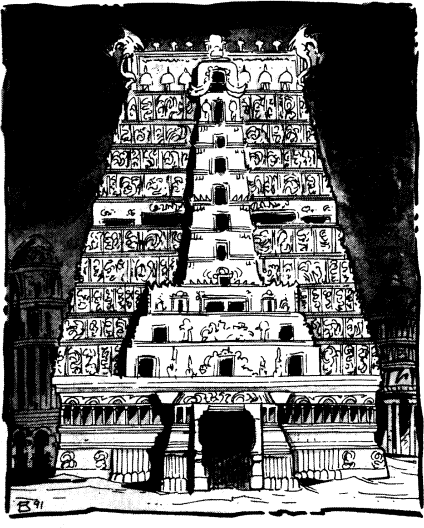
\includegraphics[width=\columnwidth]{images/tyr-1.png}
\par\textit{\small\textcopyright Wizards of the Coast, 2020.}
\end{figure}

\City{Tyr}
{15,000 (70\% humans, 10\% dwarves, 9\% half-giants, 6\% muls, 3\% elves, 1\% half-elves, 1\% other).}
{Iron, silk.}
{Common, Dwarven, Elven, Tyrian.}
{
	Located in a fertile valley in the foothills of the Ringing Mountains, it was the first city-state to successfully revolt against its sorcerer-king. King Kalak ruled Tyr until he fell to a group of heroes led by the gladiator Rikus, the wizard Sadira, and Agis of the noble house of Asticles. With Kalak dead, the High Templar Tithian stepped forward to take his place as king. Tithian received the backing of Rikus and the others, for the templar promised to free all Tyr slaves and institute other sweeping reforms---promises he actually kept. Tithian had his own agenda, of course, which slowly played out over the decade he held the throne.

	The new king created the Council of Advisers and gave members of the most important groups in Tyr a role in the city's government. Councilors were drawn from all ranks of society and worked diligently to pass laws that would strengthen Tyr's newfound freedom. Tithian allowed the Council to operate independently and virtually run the city while he sought the means to become a true sorcerer-king.

	Urik tried to capture Tyr's iron mines less than six months after Kalak's death. The resulting battles made Tyr's leaders realize how necessary a strong military was, and how important it was to resume iron production and get trade and commerce back on an even keel. During his reign, the new king also faced the problem of finding a way to overcome the Dragon's levy, had numerous skirmishes with raiding tribes, and battled angry giants intent on plundering the city. The Council struggled to stay together in the face of secret agendas and conflicting partisan interests. The templar revolt of Free Year 3 shut down the bureaucracy and public works for nearly two months until those who swore new oaths to abandon the old ways and support the tenets of Free Tyr were given more representation in the Council. The artisan strike of Free Year 6 lasted almost four months, and then ended in increased wages for basic services. Agis and the Council handled most of these crises in one way or another, for Tithian was much too busy to get involved in what he considered to be the chores of government.

	Today, in its twelfth year of freedom, Tyr faces new challenges. Agis of Asticles is dead, so his wisdom and honor can no longer guide the Council of Advisers. King Tithian's rule has come to an end. His ambitions led to his downfall, for he is trapped in the Cerulean Storm (though only a few people know of his true fate). The general populace believes that Tithian died fighting to keep Tyr free, thanks to the tales told by Rikus and Sadira. The heroes decided to keep Tithian's current state a secret, fearing that ambitious defilers might try to free him in order to gain power and prestige. Can Tyr's freedom take root in the Tablelands in the wake of these events, or will it be blown away in a devastating Tyr-storm?

	Tyr citizens remain as untroubled by modesty as they were in the days of Kalak. The less a person has to wear in the heat of the day, the better. Most wear loose-fitting cotton tunics gathered at the waist with wide, colorful belts. Others wear loincloths and vests. Light gauze or silks are draped over heads and exposed flesh to protect the skin from the blistering sun. Turbans and other forms of light headgear often finish off a Tyrian's attire.
}
{
	Four months into its twelfth year as a free city, Tyr must deal with the environmental and social conditions left over from the past decade. The Great Earthquake, for example, struck while most of Tyr's beloved heroes and its king were away. It fell to the remaining members of the Council of Advisers to pick up the pieces. Though the rumbling ground made for a terrifying period of time, Tyr escaped the disaster relatively unscathed. There was some structural damage and a small number of deaths, but most of these occurred in the Warrens. The comparatively weak and dilapidated buildings in this part of the city buckled when the quake hit, burying the residents beneath rubble and debris. Ironically, if the quake had struck during Kalak's reign, even less deaths would have occurred. In Kalak's day, the Warrens were mostly unoccupied. It's only since the First Edict freed the slaves that the Warrens have been filled to overflowing with the new crop of free citizens.

	The earthquake caused other damage. Cracks appeared in the city wall, and a whole section of the wall near the Grand Gate collapsed. Minor damage can be seen throughout the rest of the city, but the most noticeable appears on Kalak's Ziggurat. Great cracks riddle one face of the tower, while another face has collapsed into a heap of rubble. The client villages that dot the valley endured the worst of the quake's effects, however. One village was leveled by the quake, and others were pounded by rockslides that cascaded out of the mountains.

	Beyond the death and destruction, the worst aspect for the city is the refugees. Intelligent races and a wide variety of creatures and monsters have fled the mountains, flooding the valley in search of a safe haven. This, in turn, has sent villagers to the city gates, seeking protection from the ravaging hordes.

	What with the Great Earthquake, the periodic aftershocks that visit the city, and the violent Tyr-storms that occasionally sweep the land, the populace has turned into a frightened mob. Not everyone has succumbed to these base fears, of course, but a significant portion has lost control-the Council desperately needs to find a way to calm the people and restore order. A particularly vocal group claims that Kalak has returned to gain vengeance against the city, calling for open worship of the sorcerer-king to appease his wrath. Others have been trying to placate the elemental spirits of earth, hoping that they'll spare Tyr from their ground-shaking anger. Then there are those who seek to take advantage of the misfortune, looting shops, robbing nobles, and generally taking what they want and need by force of arms. These violent mobs are concentrated in the Warrens, but they sometimes range into other parts of the city to sow mayhem and destruction.

	The Council of Advisers has been working overtime to address these problems, though first it had to deal with King Tithian's supposed death. It established the OverCouncil to rule in Tithian's place so that the business of government could continue.

	Second, it increased the size of the City Guard and commanded it to restore order. Things haven't returned to normal yet, but the situation is much better than it was in the days immediately following the Great Earthquake. Various subcommittees have been set up to handle damage control, to see to the fair distribution of water and supplies, and to handle the refugee problem -both those rushing into the valley and those fleeing the villages for the safer environs of the city walls.

	The situations in the other city-states have added to the general nervousness and apprehension hanging over Tyr. While Urik has sealed itself off from the rest of the Tablelands (except for the heavily armed trade caravans that set out and return at random intervals), Gulg and Nibenay have made a few overtures to the Council of Advisers. Both city-states have offered to aid Tyr, claiming that without a sorcerer-king to defend it, the city is vulnerable to all sorts of terrible dangers. The Council, naturally, has thus far graciously refused these offers. Draj and Balic have recently resumed trade with Tyr, but both cities have changed significantly since the reported deaths of their sorcerer-kings. In fact, though Sadira and Rikus assured the Council that the kings had been disposed of by Rajaat, rumors of their return continue to drift in with caravans, adventurers, and refugees. The worst tales come out of Raam, where confusion, madness, and ambition have given rise to anarchy. Tales of nobles being murdered in their homes, of templars being slaughtered in the streets, and of vicious invaders from a hidden city-state controlled by a king named Dregoth have made the Tyr citizens ill at ease and not quite confident that their leaders can protect them.

	Sadira recently convinced a significant portion of the Veiled Alliance to come out of hiding and join Tyr society. These wizards formed a new group in Tyr, called the Preservers. The Preservers were given a place on the Council of Advisers to reflect their new role in Tyr. Sadira, as their leader and as an important member of the Council, was assigned to the OverCouncil. These good wizards are developing plans and guidelines for helping the city in a variety of ways that adhere to their overall morals and code of ethics.
}
{
\begin{figure*}[b!]
\centering
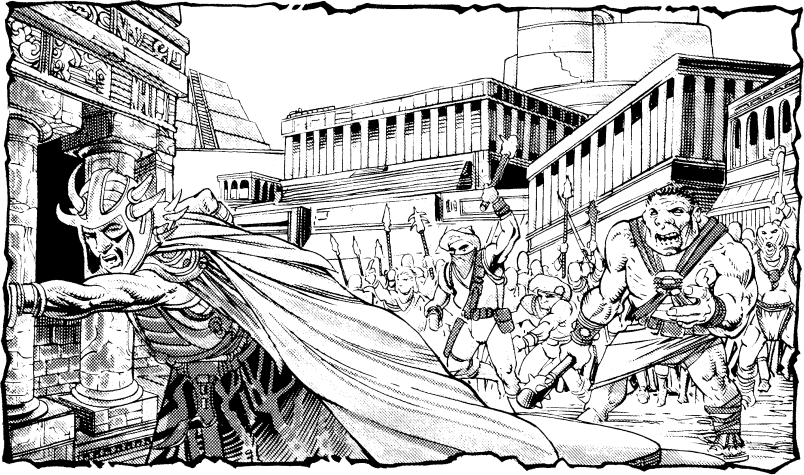
\includegraphics[width=\textwidth]{images/tyr-2.png}
\par\textit{\small\textcopyright Wizards of the Coast, 2020.}
\end{figure*}

	A Council of Advisers makes the laws of Tyr. The Council is divided into five distinct groups who together represent Tyr's varied citizenry. These groups are the Guildsmen, made up mostly of human and dwarf artisans and other professionals from Tyr's three trade districts; the Nobles, representing Tyr's aristocratic families; the Templars, who continue to handle administrative functions in the city; the Free Citizens, chosen from among the masses who were either slaves or paupers before Tyr's liberation; and the Preservers, the newest group admitted to the Council, consisting of members of the once secret and outlawed Veiled Alliance.

	When Rikus, Neeva, and Sadira returned with the news of Agis' and Tithian's death, it was resolved that the Free City shouldn't be burdened with another king. With no king to lead the city, the Council now oversees all aspects of government; a subcommittee made up of one member from each of the Council's divisions serves as an OverCouncil. This OverCouncil governs on a daily basis, while the entire Council of Advisers only meets three out of every fifteen days. The OverCouncil consists of the dwarf stonecutter Gar Bonehammer (NG male dwarf, expert 3) who represents the Guildsmen; Lady Laaj of Mycilen (LE female human, seer 6) for the Nobles; the High Templar Timor (LE male human, defiler 8) for the Templars; Rikus (NG male mul, gladiator 8/arena champion 10) who represents the Free Citizens; and Sadira (N female sun-touched half-elf, preserver 5/veiled one 5) for the Preservers.

	Surprisingly, the Council runs relatively smoothly. Some councilors posture for power and influence and partisan voting sometimes causes meetings to stall, but in general the Council has learned how to get the job done. Each division of the Council meets separately with its constituents to draft its own agenda before coming to a full session. Then the councilors do their best to get their own projects pushed through the voting process while trying to keep in mind the welfare of Tyr as a whole.

	While the Council deals with the big picture, the templars continue to fill the administrative roles they have long been associated with. Since the loss of their spellcasting abilities, it has become doubly important for this division to demonstrate why Tyr needs them. The tangled bureaucracy has been reformed, but it still exists.

	Without the templars to turn the massive wheels of government, Tyr's infrastructure would have collapsed long ago. High Templar Timor (who hides his status as a defiler) serves as the Minister of Tyr, overseeing the various Senior Templars who run departments like Fields, Finance, Public Works, Water, and Trade.
}
{
	\textbf{Free Wizards}: With preserver magic no longer outlawed in Tyr, Sadira convinced a number of preservers to come out of hiding and openly proclaim themselves to the city. As a group the free wizards are not a strong cohesive group. Individual free wizards pursue their own goals, whether in the political arena or merchant activities. Only the desire to instruct the populace in the differences between preserving and defiling magic and to build the public's trust in them unites the group.

	\textbf{House Vordon}: Under the last years of Kalak's reign, House Vordon had fallen from its position as one of the most powerful merchant houses in the Tablelands. Since the fall of Kalak, House Vordon has returned to a position of respect among its peers. The House's return to profitability is fueled by its specialization in the iron trade from the mines of Tyr.

	Thaxos Vordon is head of House Vordon. In the last ruinous days of Kalak's reign, Thaxos began a plan to overthrow the mad king. However, Kalak's demise at the hands of Rikus and the heroes of Tyr stopped him from going forward with the plan. In the years since, Thaxos has become convinced that he should become king of Tyr, and has refined the plan he originally developed for Kalak's overthrow. A number of dummy merchant houses have been created and large numbers of mercenaries hired as part of this plan. Unbeknownst to all but the highest members of House Vordon, Thaxos now has an army scattered at outposts throughout the region, waiting for his orders.

	\textbf{The Veiled Alliance}: The Veiled Alliance remains active in the wake of this new age of wizardly openness. Matthias Morthen (LG male human, preserver 8/veiled one 10) continues to lead a small number of preservers who feel that secrecy must be maintained until all of Kalak's defilers have been eradicated and the citizens of Tyr learn to deal with the responsibilities of freedom. Besides, Morthen doesn't like or trust Sadira, whom he believes has often approached the moral line between defiling and preserving magic (if not actually crossed over it) in the course of defending Tyr. He believes that the Veiled Alliance must continue, if only to serve as a balance for a wizard whose powers and motivations he doesn't fully understand.
}
{
	\textbf{Hidden Village (Thorp, 250)}: Established by the slave tribe known as the Free, the Hidden Village sits in a remote crater in the foothills of the Ringing Mountains between Tyr and Urik. Originally the tribe survived by raiding as most slave tribes do. Now the tribe has advanced into a small trading house. The villagers have developed such a strong relationship with Tyr that they have become a client village of the free city.

	\textbf{Kled (Village, 450)}: Kled is a Dwarven community that has ties to Tyr. Possibly the largest Dwarven community in the Tablelands, Kled was built near the ruins of the city of last Dwarven kings, Kemalok.

	\textbf{Mira's Halo (Thorp, 50)}: Mira's Halo is a merchant outpost owned by House Qual, one of House Vordon's dummy trading houses. The outpost is used in the iron trade between Tyr and Urik. The name of the outpost comes from an unusual rock formation nearby.
}
{
	\textbf{The Elven Market}: The Elven market is located inside the Warrens. Several nomadic Elven tribes trade at the market regularly, bringing a wide range of goods and curiosities from across the Tablelands. Many tribes own a building or two that borders on the square. Others take ownership of unoccupied buildings for the duration of their visit in Tyr. Anything can be found in the Elven market, legal or illegal. The customer just has to know the right people to ask. The market has a reputation for pick pockets and dubious merchandise, but people come from all over the city in order to find items not available anywhere else in Tyr.

	\textbf{Gladiator Stadium}: The Gladiator Arena of Tyr is the second largest building in the city, with only the ziggurat, which looms over one end of the stadium, being larger. The stadium's rectangular floor is some 90 meters long and 24 meters wide. The floor is of a hard packed sand with a reddish hue, which Tyrians say is caused by the spilling of the lifeblood of a thousand fallen gladiators. The stadium is unique in the Tyr Region as it has upper and lower seating sections. The upper section is generally referred to as ``The Sun Seats'' because of the lack of shade, and is open to the general populace. The crowd in the upper section is more raucous and enthusiastic than in the lower section. Seats in the lower section cost more and are traditionally used by merchants, and nobles.

	Despite the end of slavery in Tyr, gladiator matches are still held in the stadium. Now the bouts are not fought to the death and are open to any who wish to participate.

	The gladiator matches are only held on festival days. The remaining time, the arena floor is used for an open air market. A monthly array of tents and stalls cover the sandy floor in drunken rows. Traders who operate in these stalls offer a wide variety of legal and illegal goods and services.

	\textbf{Golden Tower}: The Golden Tower was the imperial home of the King of Tyr. Both King Kalak and King Tithian ruled from the Tower. Constructed of a rare golden granite, the tower gleams harshly during daylight. The only public entrance to the tower is to cross Tower Bridge from the Observation Tower. The public receiving areas are on the top floors, with the King's private chambers on the levels below. These included the King's library, an enormous collection of scrolls and books, many from ancient times.

	\textbf{Iron Mines}: Tyr's iron mines are the largest in the Tablelands and help the city exert leverage over the other cities in the region. The iron mines are located two days, travel northwest of the city. Death has always surrounded the mines, from cave-ins to the ``hej-kin's curse.'' The iron ore is transported to Tyr in heavily guarded caravans.

	\textbf{Kalak's Ziggurat}: The ziggurat built by Kalak still towers over the squalor of the city from its center. The ziggurat is a stepped pyramid with each level finished in a different colored glazed brick. An enormous staircase runs straight from the base to the summit of the ziggurat. Since Kalak's fall, the ziggurat has fallen into disrepair. The Great Earthquake has exacerbated this, causing an entire face of the pyramid to collapse. Great cracks riddle another face of the tower, causing concern that more of the pyramid may crumble soon. Few have dared enter the ziggurat since Kalak's death and it has become the focus of numerous rumors and frightening stories.

	\textbf{School of Thought}: The School of Thought is the only major organized institution for the study of psionics in Tyr. The school was founded a little over 30 years ago by the noblewoman Chessia. Chessia provided the funds to establish the school and made contributions to help the school operate over the years, but she is not involved running the school. The current headmistress of the School of Thought is Sycia Strimmen (NG female human, telepath 7/psiologist 9), a young and enthusiastic woman with considerable charm. She has been the headmistress for almost nine years now, since the previous headmaster, Thanik Arkos, disappeared from the school after murdering one of the master instructors. Sycia is very organized and well liked by students and instructors alike.

	\textbf{Shadow Square}: Shadow Square is a small entertainment district in the Warrens near Kalak's Ziggurat. Five lanes end at the small plaza around which sit six wineshops, a gambling house, and two hostelries. Most business in the square happens between sunset and dawn.

	\textbf{UnderTyr}: The site the city of Tyr was built on has been inhabited for thousands of years. The current city sits atop the ruins of these previous civilizations. An undercity of interconnecting byways, crumbled buildings, and dilapidated courtyards exists under the streets of modern Tyr. From buildings used as businesses to former residences and temples to forgotten gods all make up the structures of UnderTyr. It is not possible to travel from one side of the city to the other through UnderTyr. Instead pockets exist throughout the city. The location of the eight largest pockets is scattered and unconnected across the city. With names such as the Sorrows, Elven River, and Merchant's Maze, these underground locations provide opportunities for the brave or foolish. Many strange and wondrous items can be found in UnderTyr, as can dangerous creatures and malicious entities.

	\textbf{The Warrens}: The Warrens sprawl across the northern quarter of the city. The slum is filled with dilapidated structures and trash dumps. The district is filled to overflowing with the poor, mostly ex-slaves. Many are out of work, and the desperate and ambitious have chosen to prey on their neighbors. Gangs roam the Warrens targeting anyone who looks like they might have a ceramic piece. Templars and the city guard rarely patrol the Warrens anymore for fear of being overrun by the mob. Parts of the Warren are said to be cursed. Other buildings are said to be haunted or the lair of some wild beast. Anyone who enters the Warrens does so at their own peril.
}
{
	\item Slavery is outlawed in Tyr, but a group of slavers has set up a network to kidnap citizens of Tyr and sell them as slaves in other cities. The slaver network is elaborate, involving snatch teams that kidnap the victims, nobles whose estates are used to hold the captives, templars who look the other way, an Elven tribe that smuggles the slaves out of the city, and a merchant house, perhaps House Shom, that transports the captives to other cities where they are sold.
	\item Is the shadow of Kalak's ziggurat deadly? Rumors fly that ever since King Tithian's death, people are suddenly dropping dead while standing in the ziggurat's shadow. Those living close to the ziggurat are fearful of falling under what they have named Kalak's Curse. Many are fleeing, but no one knows what is causing the deaths.
	\item The elderly noblewoman Prisella Obstrunia is unlike many of her fellow nobles. Since the slaves were granted their freedom she has come to regret her past participation in the practice, and seeks to make amends somehow as she nears the end of her life. One of her former slaves, Raxenth, has remained with her as a servant and become a friend. When slavery was still in practice in Tyr, Prisella had sold off a number of Raxenth's relatives. Now, she wants to reunite Raxenth with these relatives, who through the slave trade have been scattered across the Tablelands. The noblewoman will hire the PCs to track down Raxenth's relatives and bring them back to Tyr.
	\item Zacraloc is the landlord for a large section of the Warrens, where most of the poor cannot afford to own their own homes but rent dilapidated buildings from Zacraloc. Seeking to increase his land holdings, Zacraloc uses hired thugs to set fire to a large section of the Warrens, which he does not own. His intentions are to approach the owners of those who lose their houses in the fire and offer to buy the ruined homes for very little money, since the desperate victims will need any money they can get. But the fire spreads out of control fed by either fire clerics or fire elemental creatures attracted to the original blaze.
	\item One of the rare, well-respected templars with no known enemies is found murdered. The templars are demanding better protection and seek to use the murder for political concessions by blaming the freemen. Freemen politicians reject the acquisitions but attempt to hinder the investigation, because they fear what would happen if the allegations were true. The truth is that it was not a political murder. The templar was murdered by a woman he sold into slavery years ago to merchants from Balic. The woman only recently escaped slavery during the confusion of the Wavir coup and returned to Tyr where she tracked down the person responsible for her enslavement.
	\item Tired of the raids by hej-kin on the iron mines, the Council of Advisors decides to send emissaries to the hej- kin to negotiate some sort of truce. Timor, the senior templar on the Council, does not believe the negotiations will be successful so before the PCs leave he secretly asks them to map out their journey to the hej-kin lair. With this map, a military expedition can be led to wipe out the hej- kin threat. To further complicate the PCs' mission, an agent of King Hamanu has infiltrated the mine as a guard and seeks to broker an agreement with the hej-kin on behalf of his master.
}
\begin{figure}[b!]
\centering
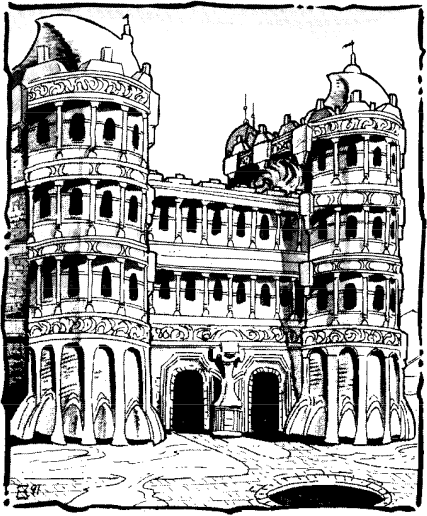
\includegraphics[width=\columnwidth]{images/urik-1.png}
\WOTC
\end{figure}

\City{Urik}
{30,000 (75\% humans, 10\% half-giants, 5\% dwarves, 3\% muls, 3\% thri-kreen, 2\% elves, 1\% halfling, 1\% other).}
{Obsidian, silk, pottery.}
{Common, Dwarven, Urikite.}
{
	Located northeast of Tyr, between the Dragon's Bowl and the Smoking Crown Mountains, the square, clean lines of the city-state of Urik can be found. The city-state has remained virtually the same as it was before the Great Earthquake and the demise of the Dragon. Hamanu, the King of the World and the Lion of Urik, was away from his city when the tremor struck.

	Although minor damage and only a few deaths resulted from the quake, the citizens trembled. When Hamanu returned, he promised his citizens that they would have nothing else to fear from Athas and its cruel temperament. The sorcerer-king's word (and his magic) was as strong as precious steel, for neither the aftershocks nor the Tyr-storm that arrived two months later could breach the towering yellow walls of Urik.

	Hamanu's promise wasn't unconditional. Though the Urikites don't have to fear change, they do have to fear their king. To disobey Hamanu is to risk punishment and even death, while to obey him is to live without fear. That's how it's always been in eternal Urik, and that's how it always will be.

	Urikites wear their hair in square cuts with elaborate ringlets. Some men wear square-cut curled beards. White linen shirts with short, tight sleeves are the fashion of Urik. Individuals of the lower classes wear plain, unadorned shirts that fall to their knees. Individuals of the upper classes increase the length to their ankles and add a striped or diamond pattern as well as a tassel-trimmed girdle. Elaborate scarves, worn only at night, indicate a citizen's station. The longer and richer the scarf, the higher the wearer's social status. By law and tradition, only templars may wear cloaks, and these are always bleached pure white for the low to mid levels and tinged yellow for the higher ranks.
}
{
	Except for the new restrictions regarding trade and travel, things in Urik are the same as they ever were. The city remains a warrior culture, ruled by a warrior king and geared toward fighting and winning wars. The current enemies aren't the other city-states, however. Rather, the refugees seeking shelter from the constant tremors and the monsters fleeing from the violent storms near the Silt Sea have become Urik's foes. When either approaches Urik's high, yellow walls, Hamanu leads his army out of his gigantic palace (called Destiny's Kingdom) and charges into battle. In most cases, the result is slaughter, for terrified invaders can't stand against Hamanu's highly trained and well-equipped legions.

	The few signs that the Great Earthquake touched Urik have been wiped out; buildings have been repaired, streets repaved, the dead buried. Now, Hamanu's magic keeps the aftershocks and the storms from entering the city, and in most respects the citizens have learned to ignore the disasters. As long as the disasters remain outside Urik's walls, the citizens see no reason to worry about them.

	Closing the city off from the rest of the world has made it difficult for certain members of Urik's society. Adventurers and traders, for example, are severely hampered by the well-guarded walls. Elves, never really welcome near Urik's walls, now avoid the city completely. They are treated like invaders, set upon as soon as they're spotted entering Urik's verdant belt. Things may change as soon as the king finishes contemplating his city's new approach to the world---or it may simply get worse if Hamanu decides to keep the rest of Athas at bay forever.
}
{
\begin{figure*}[b!]
\centering
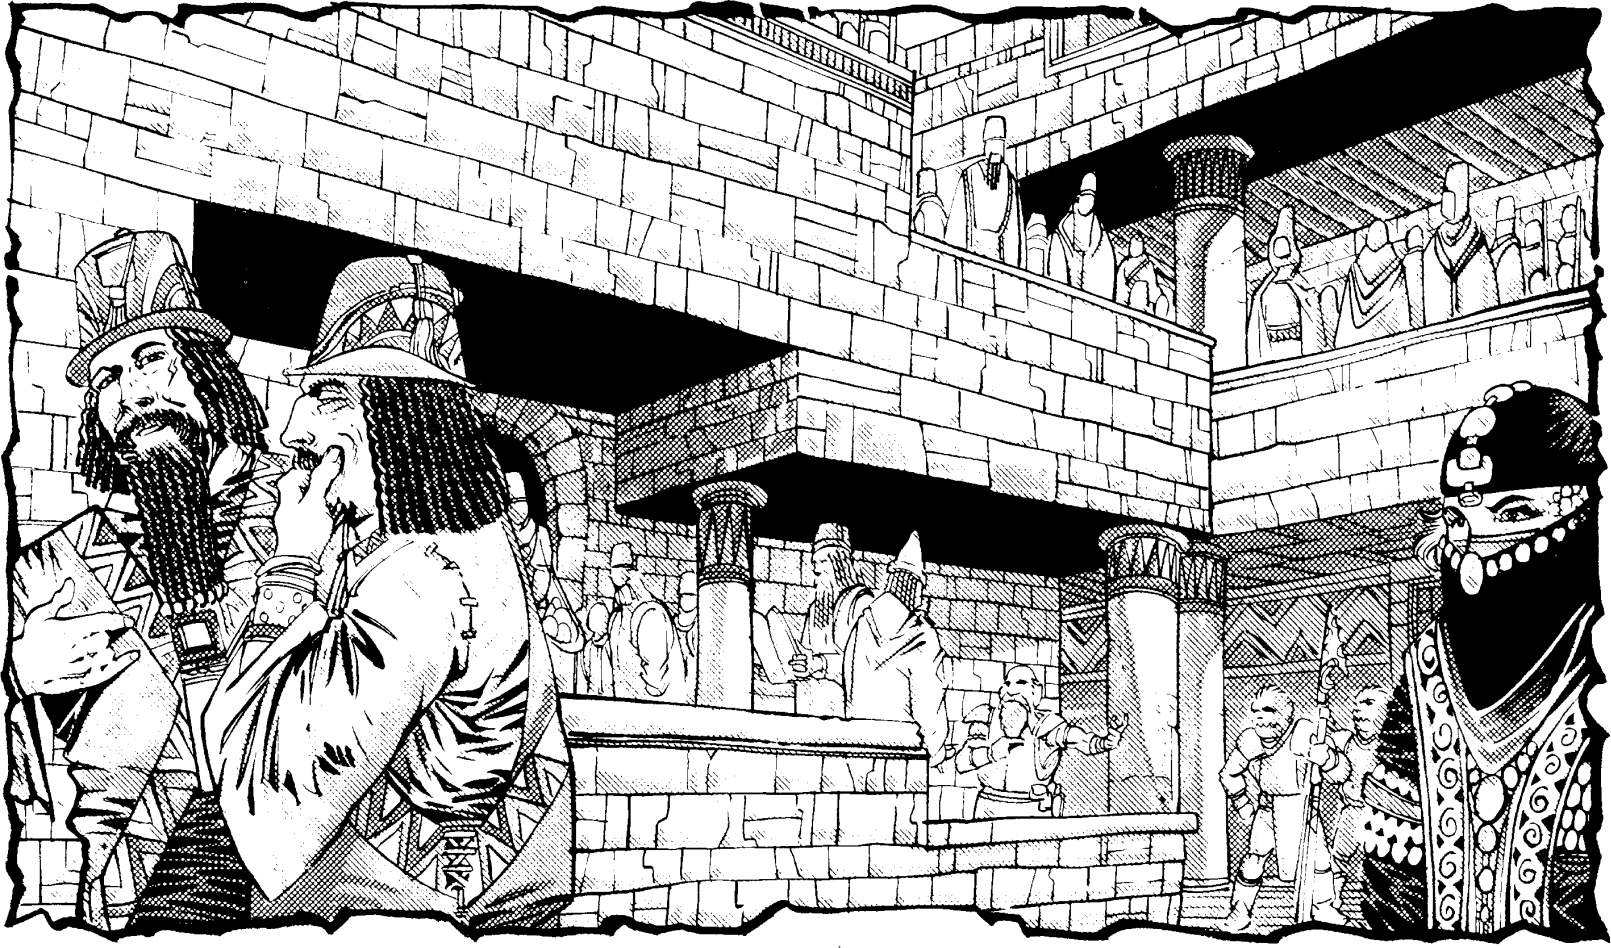
\includegraphics[width=\textwidth]{images/urik-2.png}
\WOTC
\end{figure*}

	The sorcerer-king Hamanu rules Urik, taking a personal interest in the affairs of his city. Except for Hamanu's direct involvement, Urik operates as a traditional sorcerer-king's domain. Templars enforce Hamanu's laws and handle the day-to-day bureaucracy, nobles manage the farms and water supplies, free citizens engage in business and try to remain free, and slaves provide the muscle to get everything else done.

	Hamanu is a third-stage dragon king (LE male Champion of Rajaat stage III dragon, defiler 5/psychic warrior 11/arch defiler 10/cerebremancer 5/Athasian dragon 4). Through a combination of the Way and magic, he appears before his subjects as either a tall, vigorous man with close-cropped silver hair, dark skin stretched tight over ruthless features, and heartless yellow eyes, or as a half-man and half-lion of powerful build and mythic proportions. He is never seen in his true dragon form, even by his most-trusted templars. His laws, called Hamanu's Code, are strict and innumerable, covering almost every conceivable aspect of life in Urik. Hamanu's Code relies on punishment in kind and emphasizes loyalty to the king and his templars. The Code stands unsurpassed in the Tyr Region for utility, comprehensiveness, and ruthlessness.

	At one time, Hamanu's ambitions exceeded his resources. Since the Great Earthquake and the events surrounding Rajaat's brief return, his agenda has subtly changed. The three surviving sorcerer-kings sensed that the time had come to rethink the old ways, to find new approaches to the challenges of life on Athas. Until he figures out what those new approaches are, Hamanu has decided to withdraw a bit. He has effectively closed Urik off from the rest of the Tablelands, trying to keep change from intruding on his domain for as long as possible.
}
{
	\textbf{The Brotherhood of the Mind}: The Brotherhood of the Mind is an organization of evil psionic-users that wish to overthrow the sorcerer-kings and seize power for themselves. Ruled by Liumakh, an undead psion, (NE male undead, telepath 10/thrallherd 7) the Brotherhood is headquartered in a monastery in the Smoking Crown mountains. Both Hamanu and Nibenay know of the brotherhood's existence. Nibenay seeks their destruction, while Hamanu ignores them for the most part, though he occasionally spies on the brotherhood to see if they have developed anything interesting during their psionic studies.

	\textbf{Hamanu's Halflings}: Hamanu has forged an agreement with a halfling chief from the Ringing Mountains. As long as Hamanu provides the chief with obsidian from the Urikite mines, he receives the services of 200 halfling warriors. These halflings are excellent night raiders and assassins that Hamanu has used to deadly effect in the past.

	\textbf{House Stel}: House Stel is best known for trading in the spoils of war, weapons, slaves, and various stolen cargo. Heavily influenced by the militant nature of Hamanu's regime in Urik, Stel is aggressive and confrontational with rivals. Stel caravans are heavily guarded to prevent against raids from other merchant houses, a tactic the house uses on its rivals regularly. The leaders of House Stel have a deep hatred of elves which has led to open warfare with a number of Elven tribes over the years. The House maintains lucrative trading contacts with halflings of the Ringing Mountains. Hargan Stel III (LN male human, fighter 5/rogue 2/ dune trader 5) leads the house and reflects the nature of his house, being both an expert trader and warrior.

	\textbf{The Veiled Alliance}: The Veiled Alliance has to be doubly careful in the wake of Hamanu's restrictions, and the preservers' supplies of spell components have become extremely limited. For most of the decade following the war with Tyr, Urik's Veiled Alliance was split into two factions. Its leader, the legendary Morlak, disappeared mysteriously, leaving two preservers to contend for the spot he vacated.

	When one of the contenders, Leoricius the Untamable, was killed in the Great Earthquake, the other contender worked feverishly to heal the split. This became increasingly important in the wake of Hamanu's newest restrictions. Today, Thania (LN female half-elf, preserver 5/veiled one 7) commands a whole Alliance, advocating patience and negotiation instead of the violent confrontations advocated by her one-time rival. Thania has been working to establish a partnership with Tyr's Alliance, but if Hamanu learns of it both groups will undoubtedly suffer.
}
{
	\textbf{Makla (Village, 1,000)}: The obsidian mines of Urik are located on the Mountain of the Black Crown, a peak in the Smoking Crown mountain chain. Urik's economy is completely dependent on obsidian and the tools fashioned from it. The Urikite client village of Makla serves as a base camp for the mining operations on Black Crown. The village is located on the shores of the Lake of Golden Dreams. Heavily fortified with over 500 guards, it is rarely attacked by raiders.

	\textbf{Fort Courage}: Fort Courage is a massive fortress on the trade road between Makla and Urik. This facility of House Stel is a supply point for caravans traveling between Urik and Makla and the halfling village of Ogo. Patrols are also sent from the fort to discourage raids on caravans along this route.
}
{
	\textbf{Destiny's Kingdom}: Sorcerer-King Hamanu rules Urik from his palace inside the massive fortress of Destiny's Kingdom. The walled fortress covers one square mile at the center of the city, containing troop barracks, drill fields, and an armory to support the army, as well as administrative offices for the king's templars.

	\textbf{The King's Academy}: The only legal psionic school in Urik is located within Destiny's Kingdom and is called the King's Academy. Students who attend the Academy are subject to a strict education that brings harsh punishment for failure. At the same time students are indoctrinated with the militarism that runs through the government of Urik.

	\textbf{Little Jungle}: A portion of the drill fields inside Destiny's Kingdom has been set aside for Hamanu's halfling allies to make their homes. Little Jungle is the name given to the fenced off area, where the halflings build huts in the jungle style.

	\textbf{Pit of Black Death}: Urik uses the site of an old obsidian mine for a gladiator arena, thus giving the arena its name, the Pit of Black Death. The Pit does not rise above the ground but is sunken into the ground. Stepped excavation provides viewing platforms for the crowd. All spectators must stand in the Pit, as there are no seats in the arena. The irregularly shaped combat area is made entirely of obsidian. The sun heats the black obsidian until it becomes almost unbearable for both combatants and spectators. As such most gladiator matches are held in the morning before the heat has become too great, or on rare occasions at night. Another danger of the obsidian is the thousands of sharp edges, shards, and spikes that protrude from the walls of the arena. These obsidian shards cover the walls and columns of obsidian that are scattered around the arena floor.

	\textbf{Potter's Court}: Pottery is an art form in Urik, and all other city-states recognize the superiority of Urikite pottery. The potters' workshops are collected in the Potter's Court area of the city. The concentration of so many immense kilns in the area, make Potter's Court unbearably warm, even at night when most of the potters conduct their work.

	\textbf{Potters' School}: The Potters' School is the largest group of psionic users who refuse to attend the King's Academy or register with the authorities. While the Potters' School teaches pottery casting and painting, skilled psions instruct students in the Way, outside of the influence of King Hamanu and his templars. The head instructor of the psions is Erriok (LN male human, shaper 7). He is rumored to have contact with the Veiled Alliance and work with them on occasion.

	\textbf{Three Sisters Observatory}: The Three Sisters Observatory is a two storey building with a flat roof and many observation balconies built on top of a hill called Sunrise Point. The Three Sisters Observatory served as the king's observatory until the construction of the Royal Observatory. Now the building is used to store old astronomical records and equipment, and has a run down, neglected appearance. The observatory gets its name from three identical granite hills nearby.
}
{
	\item Templars arrive at where the PCs are staying with orders to arrest them. Someone has accused the PCs of practicing magic. A fair trial is not possible and the sentence is death. The PCs must escape the templars, find out who their accuser is, and clear their name before they are captured by the templars.
	\item Unbeknownst to the PCs, their names have been added to a bounty list the templars of Urik maintain. Templars and bounty hunters begin to appear, trying to collect the bounty by capturing or killing the PCs. Whether or not the PCs are wanted by the templars, in this instance it is a case of mistaken identity. A wealthy merchant, wanted for smuggling, is supposed to be on the bounty list, however, he bribed a templar to remove his name and that of his family from the list. The PCs' names were chosen at random and added in place of the merchant's and his family to fill the vacancy.
	\item House Wavir has heard rumors that King Hamanu is planning on ordering his templars to seize all of their house's assets in Urik. Using the Wavir coup in Balic as an example, the house will be accused of planning a rebellion in Urik. Before he goes through with this threat, Hamanu is checking with the other major merchant-houses to gain their acceptance of his actions so they do not boycott his city. House Wavir gets wind of the plot and secretly plans to sneak out of the city with as much of their assets as possible. The PCs are hired to coordinate and have to safely get the Wavir agents and as much of their various assets, including wagons, merchandise, and draft animals, out of the city.
	\item The PCs are attending a feast at a noble's compound when the head of the family is murdered. Templars descend on the compound preventing anyone from leaving. Instead of investigating the crime, the templars simply state that unless the murderer is presented to them by morning everyone in the house will be executed. The PCs have until morning to find the real killer, or be executed along with everyone else.
	\item The Veiled Alliance has wondered for years about the high drik transformation process. The PCs are assigned to steal a drik egg that has undergone the process but that has not yet hatched.
	\item Saita, a templar of Urik, secretly sold some of the city's slaves to a tribe of yuan-ti in the Ringing Mountains to make some extra money. Unfortunately, the slaves were the personal property of Hamanu who is now enraged that his slaves are missing, and wants the head of the person responsible. Saita is desperate to get the slaves back before it is discovered that she is the one responsible. She secretly hires the PCs to get the slaves back from the yuan-ti any way they can.
}
\section{Beyond the Tablelands}
Plenty of action and adventure can be found across Athas. More lands of wonder, mystery, and danger exist beyond the barrenness of the Tablelands. A quick tour of these other places follows, and more information about specific locations will be revealed in future products.

\SubCity{Eldaarich}
{21,000 (85\% humans, 8\% dwarves, 4\% half-giants, 2\% muls, 1\% others).}
{Gold, silver.}
{Eldaarish, picts.}
{
\Figure*[\textwidth-2cm]{b}{images/city-eldaarich-1.png}

	Eldaarich occupies a small island in the Sea of Silt, just off the mainland. Here, isolated and protected from the rest of Athas, the citizens huddle in the paranoid delusions of their mad sorcerer-king. Daskinor, ruler of Eldaarich, believes that unknowable forces in the world are trying to destroy him.

	Every few years he puts a new name to these forces---the Order, the Veiled Alliance, Rajaat, pyreen, a merchant house, a lowly slave, or some other identifiable target becomes the imagined source of his fears for a time. Daskinor does his best to destroy these imagined enemies, and anyone who has even a passing resemblance to the target is persecuted until the next delusion grips him.

	Daskinor was never a stable ruler. From the beginning of his reign as sorcerer-king of Eldaarich, he was tormented by unfounded fears and nameless terrors that preyed upon his mind. For the first few centuries of his reign, he was able to function more or less normally despite his growing paranoia. As time passed, genuine bouts of panic began to intrude upon his psyche. These bouts lasted longer and longer, paralyzing Daskinor for hours, days, sometimes even months at a time.

	Eldaarich was constructed to protect Daskinor from his fears. Fortified walls, a strong military, devoted templars, retractable bridges, and a series of keeps and forts ensured that the entire city-state and surrounding area was secured against outsiders. Over time, it became less of a fort and more of a prison, locking king and citizens alike behind sturdy gates and high walls. Seven centuries ago, the sorcerer-king's paranoia became acute. He completely sealed his city, cutting off all ties to the other city-states. That was the way things remained until about FY 0 year, when limited trade was resumed with House Azeth of Kurn.

	Today, Eldaarich remains an isolated prison of a city. Daskinor's fears have become the fears of his citizenry, making everyone who lives under his rule as paranoid as he is. No one ever leaves Eldaarich, and no one ever enters its massive gates. It's a closed society---figuratively and literally.
}
{
	Every outsider wants to destroy their city-state and their sorcerer-king, and everyone who lives within the walls waits for an opportunity to betray you. That's what the people of Eldaarich believe, for that's what their leaders believe. Nowhere else in all of Athas is there such an underlying current of genuine, unattributable fear. It filters down from Daskinor himself, making citizen and slave alike tremble with uncontrollable paranoia.

	The citizenry is a subdued, cowering lot, given to unexpected bursts of violence once the fear inside them becomes too much to contain. In many cases, the ever-crushing weight of terror and oppression keeps the masses down, but sometimes a delusional artisan will strike out at a templar or noble, causing the level of paranoia to rise even higher.

	The quality of life isn't good in Eldaarich. Because Daskinor doesn't trust anyone, he allows his templars to dispense only the barest essentials to the free citizens and slaves. With just enough food and water to sustain them and few personal possessions, the people of the city are a sad, pathetic lot. They have no hope of a better life and no concept that a better life exists outside the walls of Eldaarich. If anyone even suggests such a notion, the ingrained fear of the unknown kicks in and makes everyone else dismiss the idea.

	While the class structure of noble, free citizen and slave exists in Eldaarich, the truth is that everyone beneath the templars is a slave to Daskinor's all-pervasive fear.

	The sorcerer-king sees threats to his rule on every face and in every dark shadow. For this reason, he permits no freedoms of any sort, not even the token rights given to the citizens of other cities. Freedom, Daskinor believes, is just an opportunity to betray his trust. So he orders his templars to oppress the people of his city, to make their lives so miserable they don't have time or strength to contemplate treachery.

	The templars don't have it much better. They're kept in line by the high templars who, in turn, are subject to Daskinor's brutal whims.

	The majority of the population consists of humans, though there are also dwarves, half-giants, and muls in significant numbers. There are also a few aarakocra wasting away in the slave pens. Daskinor has a particular hatred of the winged people and gives his templars special compensations for capturing aarakocra from the nearby White Mountains.

	If travelers were to find themselves in Eldaarich or one of its holdings (which isn't very likely), they'd feel the weight of oppression and smell the stench of mental illness that hangs in the hot, stifling air. Every year the darkness in Daskinor's soul grows deeper, his paranoia more acute. This mental deterioration is reflected in the city itself, as though each citizen were a part of the sorcerer-king's diseased mind.
}
{
	The same model of government evident in the other city-states exists in Eldaarich. The sorcerer-king Daskinor (CE male stage II Champion of Rajaat dragon defiler 8/nomad 10/cerebremancer 10/Athasian dragon 2) stands atop the societal hierarchy, his troubled delusions coloring every aspect of life in the city-state. His chaotic tendencies and often overwhelming paranoia infuse everyone he comes in contact with, making the city almost as wild and frenzied as Raam. The only thing that allows the city to function is that the citizens are a subdued lot, living in quiet fear instead of in rambunctious anarchy. Daskinor constantly watches over his shoulder for assassins that don't exist, and so do his templars and nobles. No one trusts anyone else in Eldaarich. This works out for the best, as the troubled atmosphere has fostered a society where the fear of murder and betrayal has encouraged the periodic use of such techniques by those who prefer to strike first.

	Templars and nobles regularly kill each other to keep the same from happening to them, or to gain power or position, or just because the tension of living behind heavy locks and being constantly on guard eventually drives even the most peaceful beings to violence. In Eldaarich, fears permeates everything---fear of the sorcerer-king, fear of outsiders, fear of each other, and fear of the unknown. Because the society is closed off to the rest of the world, everything on the other side of its walls and locked gates is, by definition, unknown.

	If Eldaarich is a prison, Daskinor is its most prominent prisoner. The sorcerer-king lives in a walled sub-city and rarely ventures into other parts of his realm. His constant paranoia sometimes intensifies to such a fevered pitch that he ceases to function.

	In such a state, which may last as long as months at a time, Daskinor is cared for by his senior templars. At other times, his paranoia drives him to give a name to his fear. When this occurs, the entire city mobilizes to combat this supposed threat to the realm. Currently, the use of psionic abilities has been outlawed, as Daskinor believes that the Order has initiated a campaign against his rule. Even low-powered psionicists and wild talents who openly display their abilities are subject to imprisonment or death because of the current edict. Only Daskinor, a psionicist of the highest caliber, is exempt from the terms of the edict.

	Daskinor's templars serve as administrators to the city, and also act as the sorcerer-king's eyes and ears in all corners of the domain. They are charged with watching for signs of treachery among the masses-and with dealing with such treachery before it gets out of hand. The templars are as paranoid and delusional as Daskinor, giving in to their fear whenever it overwhelms them. For this reason, Eldaarich has become a police state, and the templars are the police. They command the military. They oversee all records and the distribution of goods and services. They hold the power of life and death for the rest of the citizenry in their terrified hands.
}
{
	\textbf{Kulag:} The Kulag Order controls Daskinor's silt fleet, which currently acts as the merchant house for the Dim Lands, a nearby archipelago. It is leaded by High Templar Kerillis (LE female human, templar 14). Sometimes they also resort to piracy in the nearby islands.

	\textbf{Neshtap:} More commonly known as ``red guards'', the Neshtap are the most feared, and the second-most powerful of seven orders that Daskinor uses to maintain control of his city Eldaarich, and its client villages. They never speak, seemingly revere the element of fire, and are becoming increasingly powerful and independent from Daskinor.

	\textbf{The Veiled Alliance:} Eldaarich has no Veiled Alliance. Daskinor rooted out the Alliance and destroyed it 400 years ago when the group of preservers became his imagined enemy of the moment. Some preservers still live in the city, but they remain hidden and are relatively weak due to a lack of adequate training. Preservers from Kurn sometimes sneak into the closed city to provide training and to see what the conditions are, but they don't do this very often. If they get caught, they're put to death, and if their city of origin is discovered, it could mean war between the two cities. No one, especially Oronis the Avangion of Kurn, wants a war to break out. He does, however, feel the pain that both Daskinor and his citizens project, and often contemplates finding a solution to Eldaarich's problems.
}
{}{}
{
	\item A silt schooner owned by House M'ke was attacked and captured by the navy of Eldaarich. The merchant house could hire the PCs to raid the harbor of Eldaarich and bring the schooner back.
	\item An aarakocra from Winter Nest was captured when she flew too close to Eldaarich. The PCs are asked to free her before she is executed by the templars of Eldaarich. Once freed from her cage, the aarakocra can easily fly back to Winter Nest on her own, but the PCs will have to sneak out of Eldaarich.
	\item Grehgatha is a Kurnan preserver who has snuck into Eldaarich many times to tutor young preservers. Since she has returned from her last attempt she is consumed with freeing an entire village from Daskinor and hires the PCs to help. The PCs must come up with a way to sneak 150 people past the templars of Eldaarich.
	\item The Red Guard has become jealous of the monopoly on trade held by the templars of the Kulag Order. In an attempt to disrupt the trade negotiations, the Red Guard mounts a surprise attack on Silt Side during a meeting between Corik Azeth and High Templar Kerillis. The PCs acting as guards for House Azeth may misinterpret the attack as directed by Corik or themselves.
	\item Concerned with a recent rise in the level of the silt sea around Eldaarich, the city has declared war on all silt clerics. Mercenaries are to be hired to help hunt down the silt clerics along the coast for a hundred miles north and south of Eldaarich. The PCs could become embroiled on either side.
	\item A major giant raid on the Huuros Islands has been repulsed by the Kulag Fleet, though many casualties were suffered. Templars assign the PCs to salvage what they can from the battle, equipment as well as the bodies of those who died. Most of the wreckage is just off shore in silt 4.5 to 6 meters deep.
}


\SubCity{Kurn}
{18.000 (65\% humans, 10\% elves, 6\% muls, 6\% aarakocra, 5\% dwarves, 4\% half-elves, 3\% half-giants, 1\% other).}
{livestock, magic items, medicines.}
{Elven, Kurnan.}
{
\Figure*[\textwidth-2cm]{b}{images/kurn-1.png}
	Kurn is actually two city-states: an ancient, public metropolis, and a utopian city hidden from the rest of the world. Old Kurn sits in a lush meadow on the eastern side of the White Mountains. The trade road running north out of Draj connects Kurn to the Tyr Region, and the city welcomes merchants from the south. New Kurn lies in a fertile valley hidden among the White Mountains themselves. A secluded road protected by a towering fortress keeps the valley safe from unwanted visitors---and New Kurn doesn't want any visitors.

	Old Kurn was a prosperous but relatively small city from the Green Age that suffered great devastation in the early days of the Cleansing Wars. Once situated in a vast forest that has long since faded from the landscape, the elf city of Kurn was destroyed by the Champion called Albeorn, Slayer of Elves. When the Champions finally turned against Rajaat and became the dragon kings, the one named Keltis decided to build his city-state on the ruins of Old Kurn. He changed his name to Oronis, but decided to retain the name of the city he was building over.

	The ruins weren't in as bad a shape as Oronis originally thought. He was able to build upon many of the foundations, and a few whole structures were still fit for use. Within a decade, Oronis' Kurn was established. Within five decades, it was thriving. For five hundred years, Kurn followed the same course as the other sorcerer-king domains. Throughout that time, Oronis was troubled by something few of his peers possessed---his conscience.

	When he was Keltis, Lizard Man Executioner, he succeeded at the task Rajaat handed to him. He eliminated the entire race from the face of Athas. As the years passed and Keltis the Champion became Oronis the sorcerer-king, images of the atrocities he committed started to haunt him. After Oronis advanced to a second stage dragon king, his problems intensified. Now he had the deaths of his subjects on his head, for he had to use a specified amount of life force to power his transformation.

	He decided that none of this was what Rajaat originally promised him. Where was the restoration of the world? Athas hadn't gotten better because of the Cleansing Wars. It had gotten worse. What's more, the sorcerer-kings were continuing the downward spiral, slowly killing the world by their actions. Oronis refused to be a part of that trend any longer. He renounced his defiling skills and his status as a dragon king and sought a different path.

	That was when Kurn broke off relations with the other city-states. Mercantile activities continued, of course, but at a reduced rate. After a time, Kurn became one of the forgotten cities---just as Oronis had hoped. In the meantime, he set the next part of his plan for redemption in motion. Oronis wanted to make amends for the horrors of his past.

	The first step was to change the rules of society in Kurn. Though the city had to maintain an illusion of normalcy to keep the other sorcerer-kings from detecting treachery or weakness, Oronis secretly freed all slaves and instituted fair and just practices at all levels of society. He swore his citizens to secrecy, for if word got out he was sure his one-time peers would flock to Kurn like gith to a dying braxat. The second step was to begin construction on the utopia he envisioned. Like all ex-Champions, Oronis originally wanted to return Athas to the glory of the Blue Age.

	He decided to once more strive for that goal. In a hidden valley among the peaks of the White Mountains, the foundation stones of New Kurn were laid. As his templars and citizens worked to build New Kurn, Oronis went in search of a better path to power. Using the techniques and practices of preserving magic, Oronis looked for a way to combine magic with psionics in a more positive way than through dragon magic. It took nearly 1,000 years of study and experimentation for Oronis to develop the preserver metamorphosis spell. With it, the reformed sorcerer-king could become an advanced being aligned to goodness instead of another force for evil.

	Today, the twin cities of Kurn continue along their parallel courses. Old Kurn displays a typical sorcerer-king's domain to the other inhabitants of the region, at least on the surface, while New Kurn works to complete Oronis' experiment in regressing a small portion of Athas back through time. Between the two cities, Kurn has a total population of 18,000 people. The majority live in the new city, as each year more citizens are moved from the old city to the new. Old Kurn has such a small number of residents that it appears to be almost a ghost town, and one day Oronis plans to completely abandon it in favor of his secluded valley.
}
{
	The state of life in Kurn depends on which of the twin cities is being considered. Old Kurn, on the surface, appears to be much like any city in the Tyr Region still ruled by a sorcerer-king. Surface appearances, however, can be deceiving. Travelers who stay for any length of time might notice a few oddities. For example, the slaves seem to have a sparkle in their eyes and a bounce in their step that isn't seen in the other city-states, and templars aren't given as wide a berth as their counterparts in Urik or Nibenay. Additionally, while the merchant and tradesmen districts are always crowded, the rest of the city is as empty and desolate as the ruins of Giustenal.

	Old Kurn maintains its illusion of business-as-usual through the cooperation of its citizens and the advanced powers of its sorcerer-king. If visitors notice that the noble and templar quarters of the city are practically deserted, they usually attribute it to the rumors that Kurn is slowly dying. Dying or not, the city is far from defenseless. More than one raiding tribe has attempted to take advantage of the ``dying'' city only to discover that its defenders were more than capable of driving them off.

	Through the efforts of House Azeth and the commerce provided by other traders, Kurn maintains a modest economy. While most of the inhabitants of the Tyr Region have forgotten that this northern city exists, Kurn interacts with its closest neighbors on a regular basis. It has good relations with the aarakocra of Winter Nest, the merchants of Draj's House Tsalaxa, and the elves of a few of the local tribes. Except for the contact between House Azeth and the trade templars of Eldaarich, Kurn has little interaction with its neighboring city-state. On the other hand, Kurn sometimes has trouble with raiders from the Bandit States. The raiders don't come to the gates of the city (at least not very often), but they do attack travelers on the trade road and even plunder the client villages on rare occasions.

	New Kurn is a different matter. The high, sturdy walls of Fort Protector block the eastern entrance to the hidden valley, while the tall, steep peaks of the White Mountains make the other directions inaccessible. The only approach that might be open is by air, though flying creatures loyal to Oronis nest in the vertical peaks.

	Within the valley, Oronis' restoration project is in full swing. He has turned the valley into a place from the past, recreating the conditions of the Green Age in its sheltered space. A thick forest surrounds a lush clearing where the city of New Kurn has been built beside a small, clean lake. Oronis hopes to eventually regress the valley to conditions as they were in the Blue Age, but that's still many years away.

	The new city resembles Oronis' vision of utopia. Airy buildings with tall, elegant spires grace wide, open streets paved with white stone. Here, the people govern themselves through a system of fair laws and majority rule. Everyone has a say in the workings of the city, from the poorest laborer to the highest elected official. And if someone doesn't like the way things are going, they're free to run for a position when the current terms of office expire.

	Thanks to the fertile valley and the lush forest, no one goes hungry or thirsty in New Kurn. No creatures are hunted out of existence and no plants are plucked completely from a given area. The templars monitor the forest on a daily basis to make sure the delicate balance is maintained. For this reason, no defilers are permitted within the ranks of the templars or anywhere in the twin cities. It is strictly against the laws of Kurn to practice defiling magic.

	Oronis continues to advance as an avangion, and he tries to instill the same serene, peaceful, life-giving properties of his new form in the city and people who follow him. Where once there was a man of evil, now Oronis is a force for good in the world. His templars work to promote his plans and prepare to someday strike out from the valley with the knowledge of how to restore all of Athas. Until then, they'll work to finish the restoration of the valley and to perfect the society that Oronis has inspired.
}
{
	Oronis the Avangion (LG male Champion of Rajaat stage IV avangion, preserver 5/shaper 5/cerebremancer 10/loremaster 3/avangion 5) guides the paths of the twin cities. Oronis spent centuries redeeming himself, going so far as to change his very nature from evil to good, though he still feels he has a long way to go to make up for his acts as a Champion of Rajaat and a sorcerer-king. For this reason, he has dedicated himself and his citizens to working toward the eventual restoration of all Athas.

	While in Old Kurn, Oronis wears the guise of a normal human. In this psionically and magically induced disguise, he appears as a tall, lanky, middle-aged man with short golden hair, pale-blue eyes, and a close-cropped blond beard. He covers himself in the trappings of a sorcerer-king, wearing a golden circlet on the crown of his head and carrying an obsidian-topped walking staff. In New Kurn, however, such disguises aren't called for. There he openly displays his true avangion form---a tall, thin, hairless humanoid with golden skin, silver eyes, and gossamer wings.

	Though Old Kurn appears to run like any other city-state, Oronis long ago abandoned a monarchical form of government. He allows his subjects to govern themselves via a democratic system he developed. In this system, nobles and all citizens except templars may hold public office. Elections are held at regular intervals and term limits are set. The highest elected official is called the Presider, who sits at the head of a body called the Tribunal. Members of the Tribunal are referred to as Tribunes. Together, the Presider and the Tribunes draft the laws that keep the city-state running smoothly. The current Presider is Ulali of Prusicles (LG female half-elf, preserver 8), now in the second year of a five-year term.

	Oronis refuses to hold an official position, though he does pretend to be sorcerer-king in the old city. He acts as an adviser when the Presider or Tribunal requests his presence, but otherwise, he's more concerned with advancing as an avangion and keeping the valley restoration project on track. Oronis' templars don't serve as administrators in Kurn, either. Instead, they are the keepers and dispensers of knowledge, serving as teachers and advisers to local officials and businesses. It's also their job to oversee and handle the restoration process, under Oronis' supervision.
}
{
	\textbf{Black Brethren:} Oronis' Black Brethren are Kurn's elite army, charged with patrolling Kurn and making sure Kurn is safe and secret.

	\textbf{School of Spies:} Kurn's School of Spies is an organization of Kurnan spies, mostly female, that studies non-Kurnan societies, and brings back information to defend Kurn and improve its way of life. They have managed to infiltrate into Merchant Houses and even the templarate of every city-state in the Tablelands.

	\textbf{The Veiled Alliance:} Kurn has no Veiled Alliance. Preservers are a welcome and significant part of the society, so there's no reason for them to hide behind a veil of secrecy. In fact, preservers from other Alliance factions sometimes come to Kurn to study with Oronis. One preserver, Korgunard of Urik, even learned the steps to become an avangion and followed the path forged by Oronis. It's conceivable that more avangions will appear in the future, though when and how many is hard to say. While preservers are accepted and integral to Kurn society, defilers are considered enemies of everything Oronis stands for. The avangion is reluctant to allow his followers to make defiling magic punishable by death, as he himself was once a defiler of the highest order. However, he knows that in most cases defilers can't make the mental and spiritual changes necessary to reject that path, so he has agreed that known defilers must be banished from the society.
}
{
	\textbf{Azeth's Rest (Village, 900):} This fortified oasis and trade village lies on the trade road, reaching north from Draj to Kurn. It has remained in the hands of House Azeth ever since the trade village was founded. Fifty tough mercenaries protect it and the nearby road, manning the ballistae and fixed crossbows atop its great walls. Azeth's Rest welcomes all traders, provided they can pay the fees for using its services.

	\textbf{Silt Side (village, varies):} Silt Side is an open village on the coast of the Silt Sea. Silt Side handles trade with Eldaarich; in fact, this village is the only connection with the outside world that Eldaarich maintains. Silt Side is a seasonal village, populating and emptying for a few weeks three times every year when House Azeth members meet to trade.
}
{}
{
	\item Oronis needs many unusual spell components for his studies. Often times he does not have the time to gather all of them himself, so he hires the PCs to collect some of the rarer spell components he needs, such as roc eggshells, leather from a dune reaper matron, the bark of a zhackal, or silt eel tongues.
	\item The last time the PCs were in Kurn, they were befriended by Aloth, a friendly merchant. But now that they have returned to Kurn, Aloth has disappeared and his shop is being used by another merchant. No one claims to have heard of Aloth when the PCs ask. Has Aloth been secretly granted citizenship in New Kurn, or has something more sinister happened to him?
	\item The residents of New Kurn are up in arms when a patch of defiled ground is discovered. Suspicion falls quickly on the newest members of the community, the PCs. Actually, there is no defiler in New Kurn. The defiled ground was caused by a magical object that uses a defiling effect to power its magic. One of the preservers of New Kurn recently acquired the item and tested it, not realizing what it would do. Now he is horrified that he will be blamed for the defilement, anger Oronis, and be forbidden to practice magic, so he remains silent.
	\item The PCs have to figure out who murdered a merchant in Kurn. But the investigation is hampered when many of the witnesses and suspects disappear. Are they being relocated to New Kurn or is something more sinister happening?
	\item New Kurn needs a cistern fiend to purify its water supply. The Tribunal will greatly reward adventurers that can find and transport a cistern fiend to New Kurn.
	\item The bee keepers of Kurn are concerned. Their bees have been disappearing. Every morning the bees leave the hives and every afternoon less of the bees return. Is this some new threat from the sorcerer-king of Eldaarich or is something gathering the bees in the desert?
}
\SubCity{Pterran Vale}
{4,000 (99\% pterran, 1\% other)}
{bones tools, livestock}
{Pterran}
{
	Pterran Vale is the largest community of civilized pterrans in the Hinterlands. The buildings are lodges constructed from the bones and hides of large creatures, such as mekillots, built over hollowed out pits. Each building has steps leading down into the interior.
}
{
	The pterrans of Pterran Vale survive by hunting, farming, and herding. In addition to using bone in the construction of their buildings, they make fine bone weapons and tools.

	Each pterran must choose a life path when they come of age. There are three main Life Paths, the Path of the Warrior, the Path of the Druid, and the Path of the Psion. However, other lesser Life Paths, farmer, crafter, traders, and herders, also exist. Those pterrans following one of the lesser Life Paths are treated with respect but the three primary Life Paths are more prestigious. All leaders are in pterran society are selected from the primary Life Paths.

	The pterrans revere Athas as the Earth Mother, and their religious ceremonies and celebrations are devoted to her. After the Great Earthquake, the pterrans became convinced that the earthquake was a call from the Earth Mother to them, directing them to become more involved with the affairs of others. In response, explorers have been sent out resulting in contact with the city-state of Tyr on the other side of the Ringing Mountains. Trade routes are being established with Tyr and areas beyond.
}
{
	As in all pterran communities, Pterran Vale is lead by a Triumvirate. The Triumvirate is made up of the eldest member from each of the three primary Life Paths. The Triumvirate has the power to make all decisions for the community. However, before important decisions are made the entire community gathers to debate the question in front of the Triumvirate. Only after all pterrans have had their say does the Triumvirate make their decision.
}
{
	\textbf{Traders:} Recently, the prestige of the merchants of Pterran Vale, lead by Ptellac Goldeye, has been growing. Since they are at the forefront of the pterrans' new push to make contact with civilizations outside of their vale, the traders have become well respected. In addition, the new trade routes they have developed to the cities of the Tablelands have brought them increased wealth.

	The traders are not an organized group as yet. Thought the different merchants are business rivals some have begun to recognize their new found status and how if they united, they could exert significant influence over the pterran society of the Hinterlands.
}
{
	\textbf{Lost Scale (Small Town, 2,000):} Centuries ago, a religious dispute resulted in a schism in Pterran Vale. One group found itself in the minority and chose to leave Pterran Vale and establish their own community, and founding Lost Scale. Today the disagreement has long been settled and the two communities work together.

	Lost Scale is noted for its legion of expert pterrax riders. Each of these warriors searches rocky badlands and canyons for a pterrax egg. The baby pterrax that hatches is raised and trained from birth by its rider.
}
{}
{
	\item After the success of Ptellac Goldeye's effort to make contact with the cities of the Tablelands, the leaders of Pterran Vale have decided to send emissaries to the south, where rumors state long lost communities of pterrans exist. While the rumors are indeed true, the pterrans of the south have long ago degenerated into barbarism and cannibalism, making the expedition fraught with peril.
	\item Pterran scouts have witnessed thri-kreen with unusual coloration herding trin packs into a large enclosure in the desert. Concerned as to who these strange thri-kreen are and why they are herding trin, the leaders of Pterran Vale send the PCs to investigate.
	\item The crops in the fields around Pterran Vale are not growing as healthily as they normal do. The farmers quickly discovered why. Blood grass has sprouted up throughout the fields, stealing nutrients from the crops and attacking farmers who approach too close. Adventurers are needed to clear the blood grass from the fields, as well as discover how the blood grass came to be there in the first place.
	\item The pterrax riders of Lost Scale are having a problem locating pterrax eggs. It seems the pterrax have been driven from their normal nesting areas by an unusually large concentration of giant hornets. The pterrans hope the PCs can kill or drive off enough giant hornets to reduce the number to a balanced level so that the pterrax could return to their nesting area.
	\item The Dark One is a pterran outcast from Pterran Vale. An earth cleric, the Dark One was exiled for claiming the Great Earthquake and the aftershocks were calls from the Earth Mother demanding sacrifices of young pterrans. Now a hermit in the wilderness, the Dark One believes he has developed direct communication with the Earth Mother through a large hole in the ground. At the direction of the voice from this hole, the Dark One makes sacrifices to the Earth Mother by kidnapping and throwing pterrans into the hole. However, the Dark One is being manipulated by an earth drake, who poses as the Earth Mother to have the Dark One drop food into its lair.
	\item A pack of dune freaks have migrated to an oasis near Pterran Vale, posing a hazard to travelers going north. The PCs could be asked to clean out the dune freaks; however, they are only a lesser evil. The dune freaks were forced out of their normal hunting grounds by the increased patrols of zik-trin coming from the Great Rift.
}

\SubCity{Saragar}
{30,000 (85\% humans, 6\% elves, 6\% dwarves, 2\% other)}
{Metal weapons, puddingfish cloth, fresh water}
{Saragarian}
{
\Figure{b}{images/saragar-2.png}

	Separated from the rest of the region by the Burning Plains and the Thunder Mountains, the city of Saragar sits on the shores of the Last Sea, called Marnita by Saragarians. Visitors from the Tablelands would consider Saragar a miracle. All of the drudge work performed by slaves in other cities is taken care of by the minds of ancient criminals trapped forever in obsidian spheres. The streets are cleaned, cattle herded, crops tended, garbage removed, and water purified by these psionic powered spheres.

	The only price the citizens must pay to have all of their needs looked after in this way is that they must remain happy. The primary law of Saragar is, ``Happiness must be maintained!''
}
{
	For the most part Saragar maintains a closed self-sufficient society. To visit Saragar is to step back into the Green Age. People dress in tabards and gowns befitting a less savage age. The relatively cooler climate in the vale makes such clothing practical and comfortable. There is an abundance of metal in Saragar compared to the Tablelands, though most of it is ancient and shows signs of wear. Some new sources of ore exist in the surrounding mountains, but few citizens of Saragar still know how to extract it, let alone forge it into new items.

	Someone from the city-states of the Tyr region might consider Saragar to be a paradise. That certainly is the perception the Triune Mind Lords try to propagate. They generate laws to bolster the illusion of happiness and serenity but do nothing to truly address those concerns. The lawkeepers enforce these rules. For this reason the Saragar dwellers have learned to constantly display serene attitudes.

	There are no wizards of any sort in Saragar. Wizardry is considered evil and most citizens in Saragar who witness it don't have any idea what they are seeing. Psionics are the true power of the domain.
}
{
	The basic form of Saragar's government is a triune of 	lawmakers who write the city's laws, an army of lawkeepers to enforce the laws, and a bureaucracy of lawtenders to perform the administrative function.

	The trio that make up Saragar's Triune Mind Lords are powerful, ageless masters of psionics. They are Thesik (LE male mindlord human, kineticist 29), Barani (NE female mindlord human, telepath 28), and Kosveret (CE male mindlord elf, nomad 27). The citizens of Saragar consider the Mind Lords gods and treat them as such; thought there is little interaction between the Mind Lords and the populous.

	Senior Lawkeeper Efkenu (LN male human, psychic warrior 17) is the only person to have regular contact with the Mind Lords. He passes on their edicts and as head of the lawkeepers sees that their laws are enforced. Though a fair man, Efkenu makes no distinctions between the types of offenses and all criminal acts are punished in the same manner. The accused is taken to the harmonizers. The harmonizers are psions who reach into a subject's mind to sift and shape thoughts back to the track the Mind Lords have dictated.

	The lawkeepers are as corrupt as any templar. They enforce the laws arbitrarily and to suit their own desires. Supervisors rarely leave their offices to check on their subordinates and only rebuke subordinates for their behavior if it interferes with their own plans.

	The lawtenders perform all of the administrative work. They tend to be the most optimistic of people, determined that there is no problem that cannot be solved with a little determination and positive thinking. While they are not corrupt like the lawkeepers, the lawtenders are not very good administrators. They insist on only performing their duties by the book, and refuse to delineate from their guidelines no matter how inefficient or incorrect those guidelines are.
}
{
	\textbf{The Underground:} Despite the relative pleasantness of Saragar, there are some people who recognize that they are living in a society in decay; one that relies on powerful immortals for every aspect of their lives. These people make up the Underground which has been growing in Saragar for the past few hundred years.

	Most members of the Underground are just upset that their lives have become more inconvenient as some of the obsidian orbs have begun to fail. Others just like having someone to complain to without being arrested by the lawkeepers.

	A smaller group, who consider themselves the real Underground, speak out on street corners against the Mind Lords. They are always working on crazed schemes such as assassinating the Mind Lords, or destroying all of the obsidian orbs, but they lack the power to implement any of these plans.
}
{
	\textbf{Blufftown (Thorp, 50):} This small settlement sits on the side of a bluff on an isolated butte in the middle of the Last Sea called the Lonely Butte. The lawkeepers generally refuse to set foot on the Lonely Butte unless directly ordered to do so by the Mind Lords, which makes Blufftown a perfect safe haven for the Underground and other fugitives from the Mind Lords' rule.

	The community is little more than a couple of inns sitting inside a cave in the side of a cliff. The only way to enter the village is to be hauled up in a device consisting of a large wicker basket and a series of ropes and pulleys powered by an obsidian orb.

	\textbf{Cubarto (Small Town, 1,500):} Cubarto is located on the opposite of side of Marnita from Saragar. The people of Cubarto are loud and lusty and would not fit in Saragar. With the lack of a presence of the lawkeepers, most people in Cubarto support the Underground, though discreetly. The villagers make their living off of fishing and trade coming into their port on its way to Kharzden or Sylvandretta. The village is known throughout the valley of the Last Sea for throwing a large party at the end of the year at which a large public feast is held.

	\textbf{Kharzden (Large Town, 2,000):} Kharzden is a Dwarven colony scattered through ancient mining shafts in the Thunder Mountains. Most of the veins of ore were mined out long ago, and most of the metal items the dwarves have are ancient. The Dwarven society is matriarchal and is lead by Queen Elakta. Her word is law and is to be obeyed by all. Queen Elakta refused to have much to do with the lawkeepers, and maintains the tradition in Kharzden of not calling for help from the lawkeepers. The dwarves live underground and grow subterranean crops in massive chambers underneath the mountains. The dwarves have always doubted the power of the Mind Lords to keep the rest of the world at bay, and tried to make their community as self sufficient as possible.

	\textbf{Shallat (Hamlet, 300):} Shallat is one of a number of small fishing villagers on the shores of Marnita. What makes the village stand out is the Shallat family who rules the villages. Each member of the Shallat family is a skilled physician and many are also water clerics. The Shallat healers provide their services to anyone in need, no matter who they are. The villagers of Shallat are fun-loving people and are generally treated well by everyone living on the shores of the Last Sea. Even brigands and pirates do not harass the village, as potentially they might need the skills of the Shallat healers.

	\textbf{Sylvandretta (Small Village, 500):} The elves of Sylvandretta are called ``ghost elves'' by the people of Saragar because of their fair skin and their cold and aloof nature. The ghost elves believe that the purity of their bloodline must be preserved above all other concerns, and isolate themselves from the other races of the Last Sea region.

	The secluded settlement of Sylvandretta is located in the Spirit Forest nestled within a grove of trees of life. The community is run by a council of seven elders, elected by the general Elven population.
}
{
	\textbf{The Distillery and the Water Tower:} The distillery is a psionically powered factory used to transform salt water from the Last Sea into fresh water. The water is pumped from the distillery into the water tower which is connected to a citywide plumbing network that pipes fresh water into every building in Saragar.

	\textbf{The Palace:} A massive palace overlooks the city of Saragar from a hill east of the city. Unlike the palaces of the sorcerer-kings, the palace of the Mind Lords was built more for awe-inspiring beauty than for defense. The security provided by the lawkeepers is lax around the palace, as the Mind Lords are confident they could handle any intruder.

	Statues of the three Mind Lords stand on a circular base at the highest point of the palace. The base slowly rotates throughout the day powered by an obsidian sphere. The people of Saragar use the statues to tell time, as the statues complete a full rotation every hour.
}
{
	\item Vikus and Mylandus are two merchants who run a successful business in Saragar until Mylandus disappears with most of the funds from the business. The PCs are hired by Vikus to track down his partner. Mylandus has discovered some secret that has scared him greatly enough that he has fled the city and is trying to leave the Last Sea area completely. Unfortunately for him, Mylandus has no idea how to survive in the devastated environment of the rest of Athas and will not survive long if he is able to find a way out of the area of the Last Sea.
	\item Jarsius, a tavern owner in Saragar, has begun to have disturbing visions, in which he sees himself behaving in random acts of violence. In actuality, the visions are memories. Jarsius was an active leader of the Underground until he was captured three years ago, but his memories were erased. The effect was not perfect and now some of his suppressed memories are returning. Members of the Underground still watch Jarsius, to see if he remembers what happened to him. For Jarsius's mind was not destroyed by the lawkeepers but by members of the Underground who acted to mindwipe him to protect their identities.
	\item The lawkeepers based at South Pass discover the tracks of a large beast they have never encountered before. The PCs, as outlanders who may have seen such a beast before, are drafted to help track down the beast.
	\item A wealthy Saragarian wants to see what the world is like outside of the Last Sea. He hires the PCs to get him through the Border of Guardians.
	\item Because of the ragged appearance of most outlanders, the PCs are mistaken for druids by a small fishing community. The villagers ask the PCs for help with a school of sharks that is making fishing difficult in the area.
	\item A man is found beaten to death. His face was so badly beaten that the only way to identify him was by a letter found in his pocket. The letter was addressed from one of the PCs, and the lawkeepers wish to talk to the PC to see how he was involved with the murdered man. The PC has never heard of the man and has no idea why the dead man had the PCs name in his pocket.
}
\SubCity{Thamasku}
{12,000 (99\% rhul-thaun, 1\% other)}
{Life-shapes, fish}
{Rhul-thaun}
{
	The ancient rhul-thaun city of Thamasku sits next to Ghavin Lake a t the top of the Jagged Cliffs. The city is surrounded by a forest of hardwood trees. Like all rhul-thaun communities, the buildings are constructed of organically grown material. The architecture focuses on the vertical, with most buildings having many storeys. There is one difference from other rhul-thaun settlements. Because the city is not cramped onto a ledge of the Jagged Cliffs, the buildings of Thamasku are not crowded together allowing for wider streets and a more open feel for the city.
}
{
Rhul-thaun society is highly ritualized. Each aspect of their lives has a ritual attached to it, and throughout the day the rhul-thaun perform various rituals. Simple rituals from the greeting ritual to the payment ritual, to the before meal ritual last less than a minute, while more complex rituals such as those for legal procedures may last hours. Often the ritual is just as or more important than the associated action it is attached to, and if one of the participants makes a mistake the entire ritual is begun again. The rituals are more akin to superstitions than to a religious devotion, and allow a rhul-thaun to feel he has some control over the chaotic forces that rule his life.

As the center of the rhul-thaun society, Thamasku has a diverse population. The wealthiest rhul-thaun live side by side with the poorest of the cliff dwellers. The citizens of Thamasku are some of the few individuals on Athas who do not have to struggle daily to survive. Life-shaped devices provide a vast array of conveniences and basic needs, from nourishment to waste disposal. Most homes have indoor plumbing, operated by life-shaped engines that pump water from the lake.

Because they do not struggle daily for survival, the rhul-thaun of Thamasku have developed a rich culture of the arts and entertainment. Dance halls, theaters, art galleries, and auditoriums are numerous throughout the city, with many located in the Art Quarter on the city's eastern side.
}
{
	The rhul-thaun of Thamasku are divided into 28 different clans. The clan leaders are called Har-etuil. The Har-etuil act as judges for matters within their clans. Disputes between clans are settled by a council of Har-etuil. The collective of Har-etuil appoints the city administrator.

	Currently, Vher-asach (LN female rhul-thaun, rogue 10) holds the title of city administrator, since she inherited the position from her mother. She has proved herself a capable administrator and most expect she will remain in the position for the time being.
}
{
	\textbf{Ban-ghesh:} A guild of thieves, assassins, and hired thugs, the ban-ghesh runs the criminal activities in Thamasku. Extortion is the guild's main source of income, though their activities include burglary, smuggling, and gambling. There is little to challenge the ban-ghesh as they have a network of corrupt lawkeepers and administrative officials protecting their organization. The ban-ghesh also enters into legitimate business with merchants, providing financial support in exchange for a percentage of the merchant's profits.

	\textbf{Chahn:} The Chahn is a revolutionary organization which does not hesitate to use violence to achieve their goals. Their goal is the complete overthrow of rhul-thaun society. The Chahn are against almost every tradition in rhul-thaun society from clan-rule, the mastery of the life-shapers, to the daily rituals that dominate rhul-thaun life. The lawkeepers have branded them a terrorist group and most rhul-thaun live in fear of them.

	\textbf{Life-Shapers:} The life-shapers are a secret society that holds the knowledge of life-shaped creations. They hold a place of reverence by the rhul-thaun as the entire society is based on their works. Through the study of life-shaping the life-shapers feel a strong connection with the past back to the rhulisti, the inventors of life-shaping. The life-shapers feel they are superior to the rest of the rhul-thaun, because of this connection.

	The life-shapers guard their knowledge protectively, letting no one outside of their order learn their secrets. Because they control the creation of all life-shaped items the life-shapers can exert control over the all of the rhul-thaun, forcing the Har-etuil to listen to the life-shapers' opinions strongly.

	The life-shapers are led by Loi Far-oneth (LG male rhul-thaun, bard 7/life-shaper 5) and his chief lieutenant, Gil-ogres (LE male rhul-thaun, rogue 5/graftwarrior 7), who reside at the Sanctuary in Thamasku. Each rhul-thaun settlement has a life-shaper sanctuary with a head life-shaper who reports directly to Loi Far-oneth and his lieutenant.

	\textbf{Windriders:} Windrider is the name given to the rhul-thaun who dare to fly on the backs of various life-shaped creatures through the high winds and mist that plague the Jagged Cliff. Traveling between the rhul-thaun communities, they transport messages and merchant goods, allowing trade and communication between all their settlements. Windrider is the most glamorous position in rhul-thaun society. Though there is a windriders guild, it maintains a loose organization with little structure or hierarchy. The windriders typically work in small independent groups of 2 to 8 windriders.
}
{
	\textbf{Sol-fehn (Hamlet, 300):} Sol-fehn is a small village located at the top of a waterfall created by a river flowing from Ghavin Lake. The village serves as a hub for goods and rhul-thaun leaving Thamasku for the rest of the settlements scattered across the Jagged Cliffs. Almost all of the villagers make their living through transportation. The villagers are members of two clans that are centered in the city of Thamasku, so there is no Har-etuil in the village. An administrator appointed by the administrator of Thamasku runs the city. The current administrator is Rath-omak (LN male rhul-thaun, fighter 5).
}
{
	\textbf{Air Temple:} The air temple is located in one of the tallest of the city's spires. A dozen clerics of air staff the temple, but they have little interaction with most of the city's population. There are few devout followers in the city, and the clerics take no interest in politics. The air clerics do interact with the windriders regularly. In fact they have turned their temple into a safehome for windriders, where they can receive free food, a free room and lodging for their mounts. The clerics look on windriding as the ideal way to commune with the air spirits and treat the windriders as holy men.

	\textbf{Aviary:} The tall tower known as the aviary is home to hundreds of birds that fly about the city. The eclectic rhul-thaun known only as the Birdmaster cares for and watches over the birds. The tower is large enough for large flying creatures to roost there, and the Birdmaster allows windriders to stable their mounts at the aviary for free when in the city.

	\textbf{Conclave:} The Conclave is the meeting hall of the Har-etuil. It is a grand structure that sees little use when the Har-etuil council is not in session.

	\textbf{The Sanctuary:} The Sanctuary is the headquarters and workplace of the life-shapers in Thamasku. The mushroom shaped structure is located some 90 meters below the surface of Ghavin Lake. This masterpiece of life-shaping technology maintains fresh air within the structure by extracting it from the surrounding water through a complex gill-system. Over 150 life-shapers work at the Sanctuary creating and maintaining the life-shaped items that are used throughout Thamasku.
}
{
	\item No one has seen the Birdmaster of Thamasku for many weeks, but because of his reclusive nature, few citizens have realized this. So why are some of his birds following the PCs everywhere they go? Are the birds trying to send the PCs a message?
	\item The Ban-ghesh claim they have managed to infiltrate the Sanctuary of Thamasku and steal a wonderful new type of life-shaped item. There are rumors that the Ban-ghesh plan to sell this new item to the Chahn. The life-masters hire the PCs to recover the stolen item. The life-masters are unconcerned with the item falling into the hands of the Chahn, because there is really nothing extraordinary about the item. It is simply an unfinished common life-shaped tool. The life-masters are more concerned about the slight of someone stealing from the Sanctuary.
	\item A high-level reggelid believes that the secrets of Rajaat may be hidden in Thamasku. He has charmed a rhul-thaun climber named Bal-orean, and sent him to the rhul-thaun capital. The reggelid seeks to create a web of charmed agents throughout the city, and so has Bal-orean lure other rhul-thaun to a secluded part of the Jagged Cliffs where the reggelid has its lair. Once there the victim is charmed and sent back to Thamasku, as the reggelid attempts to create a spy network in Thamasku to root out the location of Rajaat's secrets.
	\item A wealthy benefactor hires the PCs to accompany him on a journey down the Jagged Cliffs to the Crimson Savanna to recover a long lost life-shaped artifact hidden on the Savanna. Their employer is not who he claims to be however. Taen-ofuth is really the high priest of the forbidden temple of fire in Thamasku. Frustrated with his lack of opportunity to demonstrate his devotion to his element, Taen-ofuth desires to travel to the Crimson Savanna to set a massive brush fire. He seeks to revel in the fire's destruction but also hopes to impress other rhul-thaun into seeing the benefits of devotion to the element of fire.
	\item Two weeks ago, a windrider arrived at the air temple and went immediately into a private meeting with Thim-obec, high priest of the temple. Two days later, Thim-obec left Thamasku with the windrider and a high ranking life-master on the windrider's gon-evauth. They have not been seen since, and the temple of air is seeking adventurers to find the high priest.
	\item Ghoun-awir is famous windancer, known throughout Thamasku for her daring performances. After a recent performance, a wealthy citizen claimed that Ghoun-awir is a thief and burglarized his home during her performance. The citizen's home was used as part of the performance. Ghoun-awir proclaimed her innocence before the lawkeepers arrived, but when they tried to arrest her she escaped. Since windancers wear face paint and costumes, no one is sure what Ghoun-awir really looks like. PCs could be hired to track Ghoun-awir down, or Ghoun-awir could approach the PCs to help prove her innocence by finding the true criminal.
}
\SubCity{Winter Nest}
{650 (100\% aarakocra)}
{Ice, feathers}
{Auran, Kurnan}
{
\Figure{t}{images/aarakocra-1.png}
	The village of Winter Nest is located in the frozen peaks of the White Mountains. It is the home of a civilized tribe of aarakocra.

	The unusual buildings of Winter Nest are formed from a mixture of ice, stone, and shaped bricks. To new visitors the village looks like a cluster of towers, giving the appearance that the mountain peak has a crown. There are no roads in Winter Nest and very few connecting walkways between the buildings, as the aarakocra fly rather than walk. Doorways appear all along the face of the buildings, though most are clustered near the top of each tower. Landing platforms and resting perches decorate the outsides of most building. Each tower is topped with a large rounded structure. Most of these sphere-shaped constructs are communal areas, though the highest are the personal quarters of the leaders of Winter Nest.
}
{
	The aarakocra of Winter Nest called themselves ``silvaarak,'' which means ``people of the silver wing.'' They are perceptive, and have great confidence and pride in themselves. This translates into arrogance at times, because the silvaarak believe that their ability to fly makes them superior to all other races. Though they often express sympathy for people unable to fly, this more often comes across as condescending.

	The aarakocra have had a difficult time forming friendly relations with others over the years. Only in Kurn have they made dedicated friends. Traders from Winter Nest visit the city-state of Kurn a few times each year for trade. Other attempts to make contact with other communities have meet with failure. Either due to the hostility of the natives such as in Eldaarich and the Bandit States, or the silvaarak's condescending nature towards other races.
}
{
	Winter Nest is lead by Traaka (LG female aarakocra, air cleric 5/elementalist 2) a female aarakocra of many years. Traditionally, the aarakocra are isolationists, and Traaka supports this policy. The isolationist policy was adopted years ago after bad experiences with Eldaarich and later with the peoples of the Bandit States. The policy has kept the village safe over the years and most of the silvaarak want to see it continue.

	However, many of the younger generation of bird-people desire to explore the world beyond the White Mountains. They have been vocal in their wish to explore and make contact with other civilizations, believing they will not experience such bad receptions as those the aarakocra received in Eldaarich or the Bandit States. Pointing to Kurn, these young bloods believe there is opportunity for the silvaarak in positive relationships with outsiders.

	Traaka understands the young aarakocra's desires, but wishes to maintain the status quo for the protection of the village. She is trying to develop a middle path that would allow some exploration without making the location of the village well known to its enemies.
}
{
	\textbf{Air Clerics:} Winter Nest is ruled by clerics of Air and Ice drawn from the leading aarakocra families. The clerics meet in a large hall in Winter Nest to discuss community issues; when there is a particularly contentious debate, the priests adjourn to the very summit of a nearby mountain overlooking the village. There, perched on the ice and surrounded by the sky, the priests of the two faiths pray for guidance together.	
}
{}
{
	\textbf{Air Temple:} The Air Temple is the grandest structure in the village. The temple is built like a huge brazier, with four legs made of massive evergreen tree trunks dragged up from the foothills centuries ago. These tree boles, each more than 30 meters long, are set in the icy ground and canted to nearly join at the tops. There is a concave plate of ice, 6 meters in diameter, held up between the four posts with a hole 2.5 meters in diameter cut in its center. Priests of Air preach from the center of the bowl, while congregants gather on the rim of the bowl and on the perches placed at intervals along the legs.

	\textbf{Ice Temple:} Smaller only to the Air Temple, the Ice Temple (which is basically another word for water at such high altitudes most of the year) is built of large sheets of translucent white and blue ice, layered upon one another to create a five-sided pyramid more than 10 meters tall. The interior is sunken below ground level dug into the glacier so all the worshippers are surrounded by primordial ice throughout the services. Fresh plates of ice are added to the temple throughout the High Sun.
}
{
	\item Few in Winter Nest took much notice when a roc landed on a perch overlooking the village. Two days later the roc has been joined by a dozen more of his kind. The large birds rarely move from their perches, but their menacing presence is unnerving the aarakocra of Winter Nest.
	\item The wind patterns around Winter Nest have changed drastically. A dangerous downdraft has developed making any attempt at flying from the village fraught with peril. Town elders are puzzled by this sudden change, and have forbidden all but the strongest, most agile fliers from leaving Winter Nest. Air clerics are calling for a sacrifice to appease the air spirits, but the town elders want to understand what is going on before they decide, and the local druid who communes with the spirit of the land has disappeared.
	\item The aarakocra of Winter Nest tell tales of a wise old aviarag named Vocia that lives in a cave near the base of the White Mountains. The noble beast has not been seen for three years. Templars from Eldaarich, intent on plundering Vocia's lair, have been spotted approaching the cave. Traaka needs volunteers to warn Vocia. Unfortunately Vocia has passed away due to old age, leaving the PCs to defend her cave, as well as her remains, which the templars wish to plunder.
	\item A defiler has polymorphed himself into an aarakocra and infiltrated Winter Nest, seeking to gain some of the knowledge from the preservers of Winter Nest. His defiling is having an adverse affect on the ice sculpted portions of Winter Nest's buildings. If he is not unmasked soon, one or more buildings in the community may collapse.
	\item Some of the more adventuresome young aarakocra enjoy a deadly challenge. They know of a lair of an air drake on one of the other mountains in the White Mountain range. To show their bravery they occasionally sneak into the lair and come back with a scale or other souvenir. The act is not as dangerous as it sounds, since the aarakocra know the air drake's migration pattern and typically know when it is not in this particular lair. Some of these youths could challenge the PCs to try this stunt, but unfortunately for the PCs the air drake has returned to the lair earlier than expected in order to lay eggs.
	\item A heavily armed Tsalaxan caravan has arrived at the foot of the White Mountains from Draj. The Tsalaxans seem to be trying to reach Winter Nest but the steep mountain sloop prevents them from approaching from below. They have not given up and continue to search for some path up the mountain to Winter Nest. The aarakocra believe the Tsalaxans are raiders and wish to avoid them. The Winter Nesters know their village cannot be reached except through the air, and are not concerned that the Tsalaxans will be able to reach the village. However, Traaka wishes to determine the caravan master's true intentions in case the aarakocra are mistaken. PC allies of the aarakocra could infiltrate the caravan while not obviously tying directly back to the aarakocra.
}
